%%% The main file. It contains definitions of basic parameters and includes all other parts.

%% Settings for single-side (simplex) printing
% Margins: left 40mm, right 25mm, top and bottom 25mm
% (but beware, LaTeX adds 1in implicitly)
\documentclass[12pt,a4paper]{report}
\setlength\textwidth{145mm}
\setlength\textheight{247mm}
\setlength\oddsidemargin{15mm}
\setlength\evensidemargin{15mm}
\setlength\topmargin{0mm}
\setlength\headsep{0mm}
\setlength\headheight{0mm}
% \openright makes the following text appear on a right-hand page
\let\openright=\clearpage

%% Settings for two-sided (duplex) printing
% \documentclass[12pt,a4paper,twoside,openright]{report}
% \setlength\textwidth{145mm}
% \setlength\textheight{247mm}
% \setlength\oddsidemargin{14.2mm}
% \setlength\evensidemargin{0mm}
% \setlength\topmargin{0mm}
% \setlength\headsep{0mm}
% \setlength\headheight{0mm}
% \let\openright=\cleardoublepage

%% Generate PDF/A-2u
\usepackage[a-2u]{pdfx}

%% Character encoding: usually latin2, cp1250 or utf8:
\usepackage[utf8]{inputenc}
\usepackage[T1]{fontenc}
\usepackage{textcomp}

%% Prefer Latin Modern fonts
\usepackage{lmodern}

%% Further useful packages (included in most LaTeX distributions)
\usepackage{amsmath}        % extensions for typesetting of math
\usepackage{amsfonts}       % math fonts
\usepackage{amsthm}         % theorems, definitions, etc.
\usepackage{bbding}         % various symbols (squares, asterisks, scissors, ...)
\usepackage{bm}             % boldface symbols (\bm)
\usepackage{graphicx}       % embedding of pictures
\usepackage{fancyvrb}       % improved verbatim environment
\usepackage{natbib}         % citation style AUTHOR (YEAR), or AUTHOR [NUMBER]
\usepackage[nottoc]{tocbibind} % makes sure that bibliography and the lists
			    % of figures/tables are included in the table
			    % of contents
\usepackage{dcolumn}        % improved alignment of table columns
\usepackage{booktabs}       % improved horizontal lines in tables
\usepackage{paralist}       % improved enumerate and itemize
\usepackage{xcolor}         % typesetting in color

\usepackage{caption}
\usepackage{subcaption}

\usepackage{tikz}
\usetikzlibrary{shapes, arrows}

\usepackage{dirtytalk}

\usepackage{threeparttable}

\usepackage{fancyvrb}

\usepackage{cleveref}
\Crefname{appendix}{Attachment}{Attachments}

\usepackage{enumitem}
\setlist[enumerate]{itemsep=0mm}
\setlist[itemize]{itemsep=0mm}

\usepackage{footmisc}

%%% Basic information on the thesis

% Thesis title in English (exactly as in the formal assignment)
\def\ThesisTitle{Generating a drawing according to a textual description}

% Author of the thesis
\def\ThesisAuthor{Peter Grajcar}

% Year when the thesis is submitted
\def\YearSubmitted{2021}

% Name of the department or institute, where the work was officially assigned
% (according to the Organizational Structure of MFF UK in English,
% or a full name of a department outside MFF)
\def\Department{Institute of Formal and Applied Linguistics}

% Is it a department (katedra), or an institute (ústav)?
\def\DeptType{Institute}

% Thesis supervisor: name, surname and titles
\def\Supervisor{Mgr. Rudolf Rosa, Ph.D.}

% Supervisor's department (again according to Organizational structure of MFF)
\def\SupervisorsDepartment{Institute of Formal and Applied Linguistics}

% Study programme and specialization
\def\StudyProgramme{Computer Science}
\def\StudyBranch{Programming and Software Systems}

% An optional dedication: you can thank whomever you wish (your supervisor,
% consultant, a person who lent the software, etc.)
\def\Dedication{
I would like to thank my supervisor Mgr. Rudolf Rosa, Ph.D., for his advice and help. Furthermore, I would like to thank my colleagues and friends Katarína Dan\v{c}ejová and Jakub \v{C}atlo\v{s} for reviewing the text of this thesis and others who helped me throughout the course of my studies.
}

% Abstract (recommended length around 80-200 words; this is not a copy of your thesis assignment!)
\def\Abstract{%
Text-to-image generators have improved significantly with the recent development of deep neural networks. However, generating complex scenes with multiple objects and relations still remains a difficult problem. In this thesis, we implement a text-to-drawing generator using scene graphs as an intermediate structure. We focus on determining object size and position given a scene graph. We propose a rule-based and classifier-based approach to determine the object position and multiple approaches for size extraction from the scene graph dataset. We provide details of our implementation. We compare and evaluate our approaches and present the results. Finally, we propose potential future use in photorealistic text-to-image generation.
}

% 3 to 5 keywords (recommended), each enclosed in curly braces
\def\Keywords{%
{natural language processing} {image generation} {scene graphs}
}

%% The hyperref package for clickable links in PDF and also for storing
%% metadata to PDF (including the table of contents).
%% Most settings are pre-set by the pdfx package.
\hypersetup{unicode}
\hypersetup{breaklinks=true}

% Definitions of macros (see description inside)
%%% This file contains definitions of various useful macros and environments %%%
%%% Please add more macros here instead of cluttering other files with them. %%%

%%% Minor tweaks of style

% These macros employ a little dirty trick to convince LaTeX to typeset
% chapter headings sanely, without lots of empty space above them.
% Feel free to ignore.
\makeatletter
\def\@makechapterhead#1{
  {\parindent \z@ \raggedright \normalfont
   \Huge\bfseries \thechapter. #1
   \par\nobreak
   \vskip 20\p@
}}
\def\@makeschapterhead#1{
  {\parindent \z@ \raggedright \normalfont
   \Huge\bfseries #1
   \par\nobreak
   \vskip 20\p@
}}
\makeatother

% This macro defines a chapter, which is not numbered, but is included
% in the table of contents.
\def\chapwithtoc#1{
\chapter*{#1}
\addcontentsline{toc}{chapter}{#1}
}

% Draw black "slugs" whenever a line overflows, so that we can spot it easily.
\overfullrule=1mm

%%% Macros for definitions, theorems, claims, examples, ... (requires amsthm package)

\theoremstyle{plain}
\newtheorem{thm}{Theorem}
\newtheorem{lemma}[thm]{Lemma}
\newtheorem{claim}[thm]{Claim}

\theoremstyle{plain}
\newtheorem{defn}{Definition}

\theoremstyle{remark}
\newtheorem*{cor}{Corollary}
\newtheorem*{rem}{Remark}
\newtheorem*{example}{Example}

%%% An environment for proofs

\newenvironment{myproof}{
  \par\medskip\noindent
  \textit{Proof}.
}{
\newline
\rightline{$\qedsymbol$}
}

%%% An environment for typesetting of program code and input/output
%%% of programs. (Requires the fancyvrb package -- fancy verbatim.)

\DefineVerbatimEnvironment{code}{Verbatim}{fontsize=\small, frame=single}

%%% The field of all real and natural numbers
\newcommand{\R}{\mathbb{R}}
\newcommand{\N}{\mathbb{N}}

%%% Useful operators for statistics and probability
\DeclareMathOperator{\pr}{\textsf{P}}
\DeclareMathOperator{\E}{\textsf{E}\,}
\DeclareMathOperator{\var}{\textrm{var}}
\DeclareMathOperator{\sd}{\textrm{sd}}

%%% Transposition of a vector/matrix
\newcommand{\T}[1]{#1^\top}

%%% Various math goodies
\newcommand{\goto}{\rightarrow}
\newcommand{\gotop}{\stackrel{P}{\longrightarrow}}
\newcommand{\maon}[1]{o(n^{#1})}
\newcommand{\abs}[1]{\left|{#1}\right|}
\newcommand{\dint}{\int_0^\tau\!\!\int_0^\tau}
\newcommand{\isqr}[1]{\frac{1}{\sqrt{#1}}}

%%% Various table goodies
\newcommand{\pulrad}[1]{\raisebox{1.5ex}[0pt]{#1}}
\newcommand{\mc}[1]{\multicolumn{1}{c}{#1}}

\newcommand*{\fullref}[1]{\hyperref[{#1}]{\Cref{#1} \nameref*{#1}}}

\DeclareMathOperator{\argmax}{argmax}


% Title page and various mandatory informational pages
\begin{document}
%%% Title page of the thesis and other mandatory pages

%%% Title page of the thesis

\pagestyle{empty}
\hypersetup{pageanchor=false}
\begin{center}

\centerline{\mbox{
\includegraphics[width=166mm]{./figures/logo-en.pdf}}}

\vspace{-8mm}
\vfill

{\bf\Large BACHELOR THESIS}

\vfill

{\LARGE\ThesisAuthor}

\vspace{15mm}

{\LARGE\bfseries\ThesisTitle}

\vfill

\Department

\vfill

{
\centerline{\vbox{\halign{\hbox to 0.45\hsize{\hfil #}&\hskip 0.5em\parbox[t]{0.45\hsize}{\raggedright #}\cr
Supervisor of the bachelor thesis:&\Supervisor \cr
\noalign{\vspace{2mm}}
Study programme:&\StudyProgramme \cr
\noalign{\vspace{2mm}}
Study branch:&\StudyBranch \cr
}}}}

\vfill

% Zde doplňte rok
Prague \YearSubmitted

\end{center}

\newpage

%%% Here should be a bound sheet included -- a signed copy of the "bachelor
%%% thesis assignment". This assignment is NOT a part of the electronic
%%% version of the thesis. DO NOT SCAN.

%%% A page with a solemn declaration to the bachelor thesis

\openright
\hypersetup{pageanchor=true}
\pagestyle{plain}
\pagenumbering{roman}
\vglue 0pt plus 1fill

\noindent
I declare that I carried out this bachelor thesis independently, and only with the cited
sources, literature and other professional sources. It has not been used to obtain another
or the same degree.

\medskip\noindent
I understand that my work relates to the rights and obligations under the Act No.~121/2000 Sb.,
the Copyright Act, as amended, in particular the fact that the Charles
University has the right to conclude a license agreement on the use of this
work as a school work pursuant to Section 60 subsection 1 of the Copyright~Act.

\vspace{10mm}

\hbox{\hbox to 0.5\hsize{%
In \hbox to 6em{\dotfill} date \hbox to 6em{\dotfill}
\hss}\hbox to 0.5\hsize{\dotfill\quad}}
\smallskip
\hbox{\hbox to 0.5\hsize{}\hbox to 0.5\hsize{\hfil Author's signature\hfil}}

\vspace{20mm}
\newpage

%%% Dedication

\openright

\noindent
\Dedication

\newpage

%%% Mandatory information page of the thesis

\openright

\vbox to 0.5\vsize{
\setlength\parindent{0mm}
\setlength\parskip{5mm}

Title:
\ThesisTitle

Author:
\ThesisAuthor

\DeptType:
\Department

Supervisor:
\Supervisor, \SupervisorsDepartment

Abstract:
\Abstract

Keywords:
\Keywords

\vss}

\newpage

\openright
\pagestyle{plain}
\pagenumbering{arabic}
\setcounter{page}{1}

%%% A page with automatically generated table of contents of the bachelor thesis

\tableofcontents

%%% Each chapter is kept in a separate file
\chapter*{Introduction}
\addcontentsline{toc}{chapter}{Introduction}

This thesis aims to implement a drawing generator capable of generating complex scenes for given textual descriptions of the scenes. Generating drawings is substantially less ambitious than generating photorealistic images. However, the problem still poses multiple challenges whose solutions may also be useful in photorealistic image generation. 

\medskip

Despite the significant progress in the field of text-to-image generation, these generators still struggle with more complex scenes. Many approaches only work on limited domains \citep{zhang2017stackgan}. While promising achievement in a zero-shot text-to-image generation has recently been made \citep{ramesh2021zeroshot}, generating complex images remains a challenge. One fairly recent approach \citep{johnson2018image} uses a scene graph representation of the scene in an attempt to address the challenges of complex image generation with many objects and relations. The scene graph is a structure that represents the relations and objects in the form of a directed graph. The scene graph is used as an intermediate structure. However, generating a scene graph from a natural language and generating images from the scene graphs are still complex tasks. 

\medskip

Our work focuses on determining the spatial properties (the position and the size) of the objects within the scene. We propose multiple approaches and compare them. Our approaches may serve as an alternative to box regression methods used in existing scene graph based text-to-image generation \citep{johnson2018image,tripathi2019using}. Limiting ourselves to generating drawings allows us to use an existing dataset of hand-drawn images of common objects such as \emph{Quick, Draw!} \citep{quickdraw}. We also implement a rule-based description processing that converts text to a scene graph based on the syntactic analysis.

\medskip

While we are limited to drawings in this thesis, the proposed approaches for determining the positions and sizes could be used for layout generation. The layout is a bounding box corresponding to an object in the scene, which may also be used for image generation \citep{zhao2019image}. 

\medskip

This thesis is structured into six chapters. The first chapter provides an overview of recent text-to-image generators, work related to scene graphs, and drawing datasets. The second chapter introduces our approach for drawing generation. In the third chapter, we provide details of the implementation of our approach presented in the second chapter. The next chapter contains brief instructions for users of our implementation. The fifth chapter presents the results of our approaches for determining spatial properties of objects. The chapter is followed by a discussion of the results and a general conclusion.

\chapter{Related Work}

\section{Text-to-Image Generation}

Most of the recent research on text-to-image generators has focused on generating photorealistic images \citep{zhang2017stackgan,ramesh2021zeroshot,johnson2018image,zhao2019image,mansimov2015generating,oord2016conditional,oord2016pixel,reed2016learning} using machine learning approaches such as Generative Adversarial Networks -- GANs \citep{zhang2017stackgan,zhao2019image}, Cascaded Refinement Networks -- CRNs \citep{johnson2018image} or autoregressive models \citep{ramesh2021zeroshot,oord2016conditional,oord2016pixel}.
However, these models are limited to generating low-resolution images, e.g., $32\times32$ \citep{mansimov2015generating,oord2016conditional,oord2016pixel}, $64\times64$ \cite{johnson2018image,oord2016pixel}, $128\times128$ \citep{reed2016learning}, $256\times256$ \citep{zhang2017stackgan,ramesh2021zeroshot}. Some approaches do not generate images directly from the text but use intermediate structures such as scene graphs \citep{johnson2018image,tripathi2019using} or layouts \citep{zhao2019image}. 

\begin{figure}[ht]
    \centering
    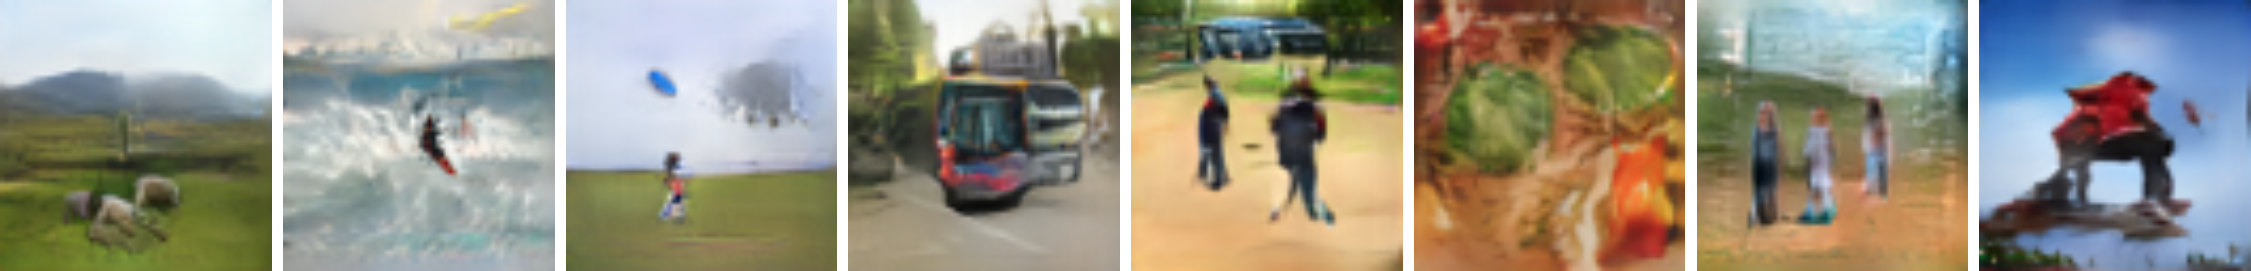
\includegraphics[width=\textwidth]{figures/johnson.png}
    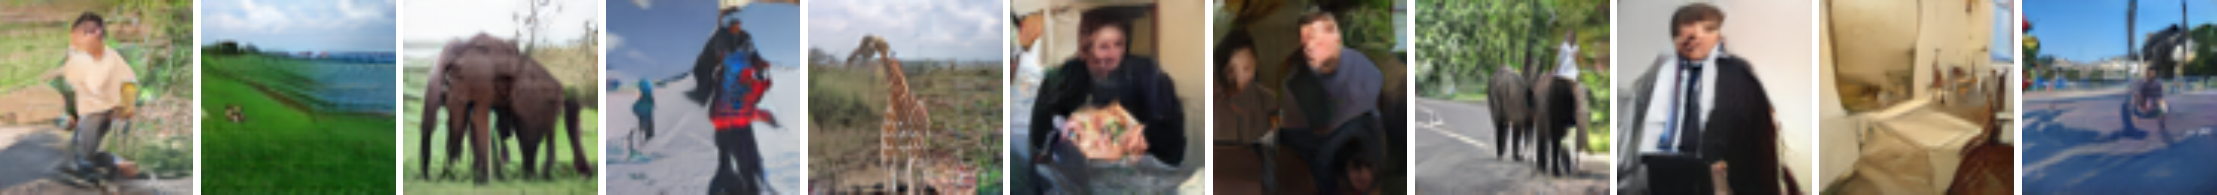
\includegraphics[width=\textwidth]{figures/zhao.png}
    \caption[Generated photorealistic images]{Examples of generated photorealistic images. Top row: Johnson et al. \cite{johnson2018image}, bottom row: Zhao et al. \cite{zhao2019image}.}
    \label{fig:photorealistic_examples}
\end{figure}


\section{Scene Graphs}

A scene graph is a graph-based representation of a scene, where vertices of the graph are objects and edges are relations between objects. Scene graphs have been used for image retrieval \citep{schuster2015generating,johnson2015image}, image generation \citep{johnson2018image}, improving \citep{Liu_2017} or evaluating \citep{anderson2016spice} image captions. Schuster et al.  \citep{schuster2015generating}, proposed rule-based and \break classifier-based approaches for converting sentences to scene graphs with no significant performance difference between the two. We use our own yet similar rule-based approach for text-to-scene graph conversion.

\begin{figure}[ht]
    \centering
    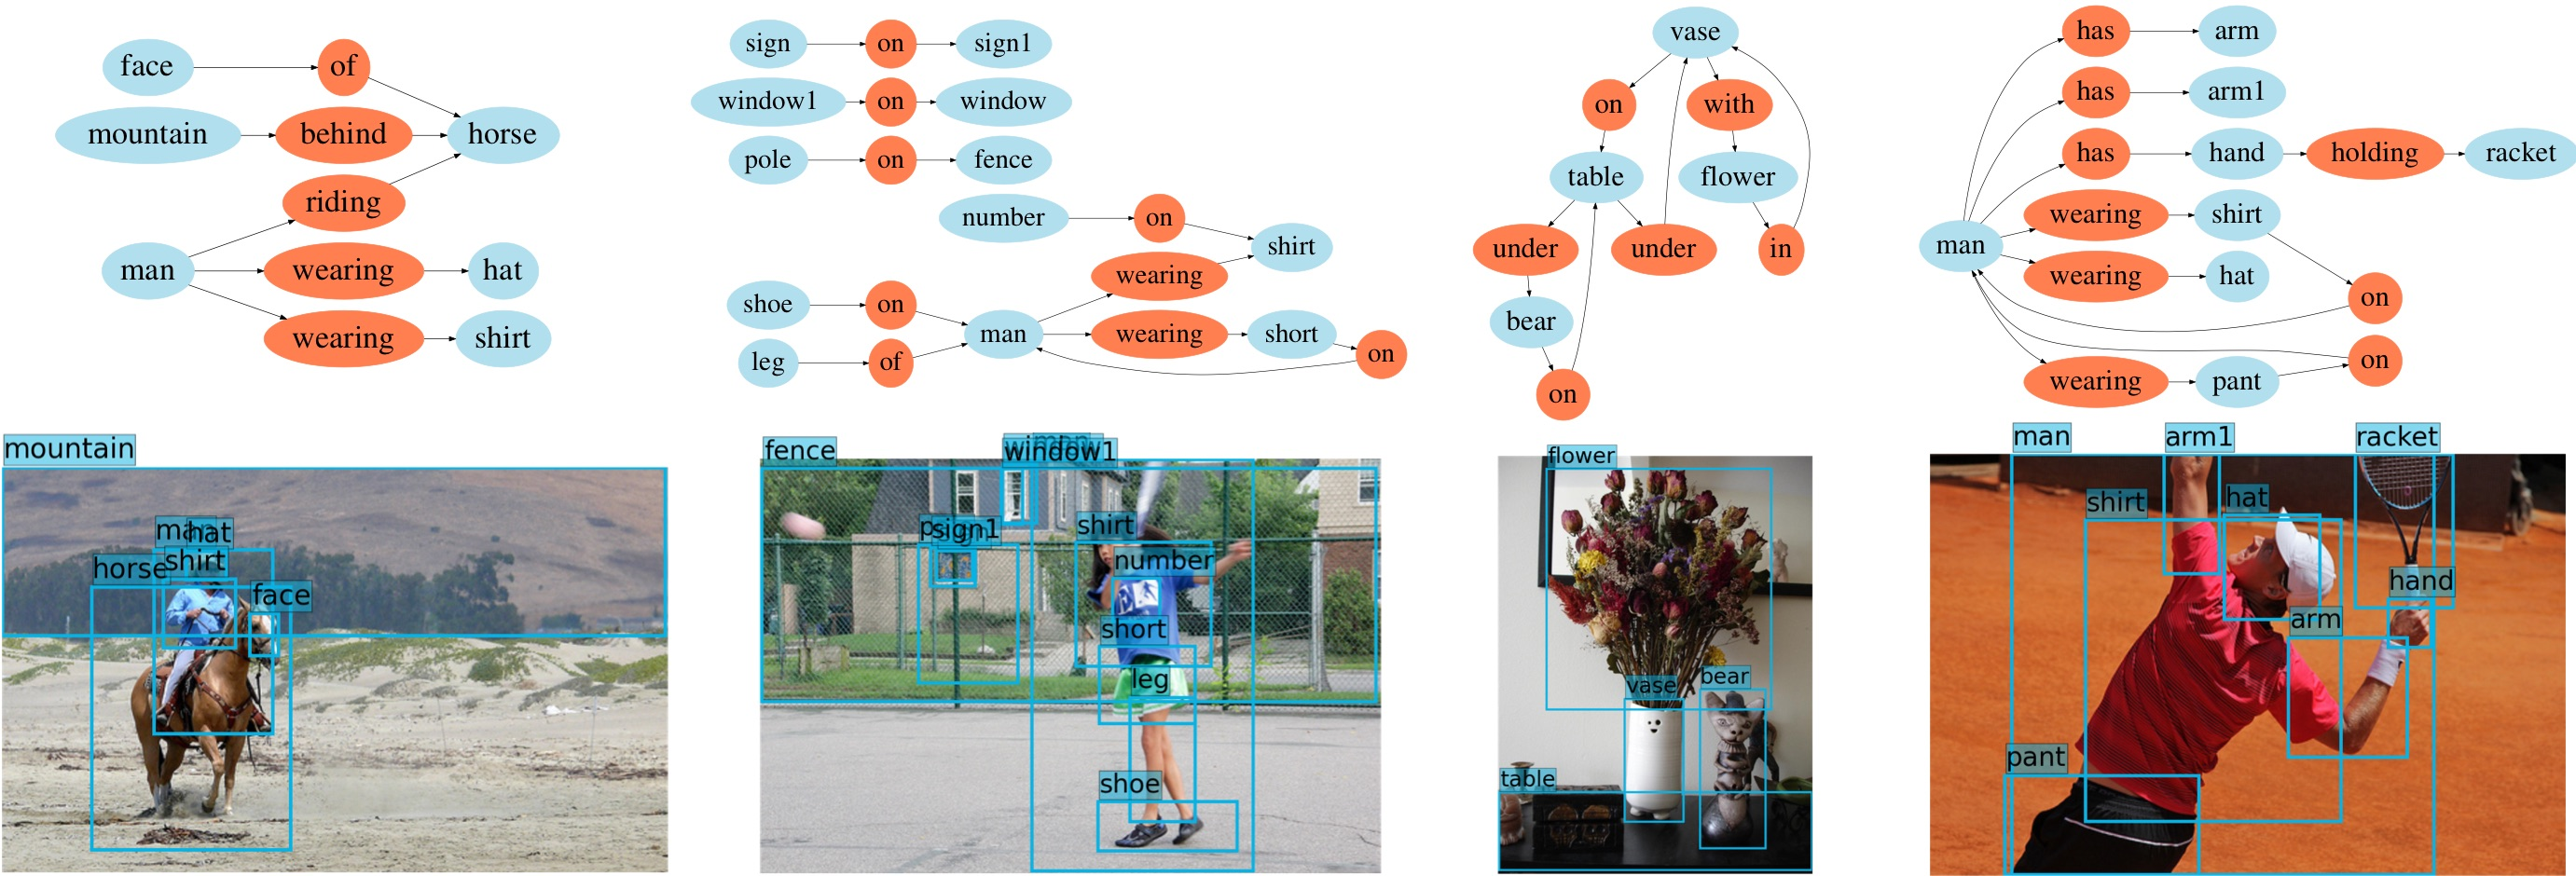
\includegraphics[width=\textwidth]{figures/scene_graph.jpeg}
    \caption[Examples of scene graphs]{Examples of scene graphs from the \emph{Scene Graph} dataset.\footref{footnote:quickdraw} \citep{xu2017scenegraph}}
    \label{fig:scene_graph_example}
\end{figure}
\addtocounter{footnote}{1}
\footnotetext{Image taken from the \emph{Scene Graph} dataset webpage \url{https://cs.stanford.edu/~danfei/scene-graph/}.\label{footnote:quickdraw}}

\medskip

Most work on scene graphs is based on \emph{Visual Genome}  \citep{krishnavisualgenome} dataset, which contains scene graphs annotated by humans. This thesis uses \emph{Scene Graph}  \citep{xu2017scenegraph} dataset based on the \emph{Visual Genome}. Unlike the original dataset, this dataset is deprived of ambiguous object names and poor quality bounding boxes.

\section{Drawing Datasets}

Google's \emph{Quick, Draw!} \citep{quickdraw} dataset is the largest hand-drawn sketch dataset at the time. It contains 50 million individual drawings classified into 345 categories. The \emph{Quick, Draw!} dataset provides the broadest range of categories compared to other widely used datasets such as \emph{TU-Berlin} \citep{eitz2012hdhso} dataset with 250 categories and \emph{Sketchy} \citep{sketchy2016} dataset with 125 categories.

\medskip

The \emph{Quick, Draw!} \citep{quickdraw} dataset contains sketches of common objects represented as sets of pen strokes. \Cref{fig:quickdraw_example} shows a sample of sketches present in the dataset.

\begin{figure}[ht]
    \centering
    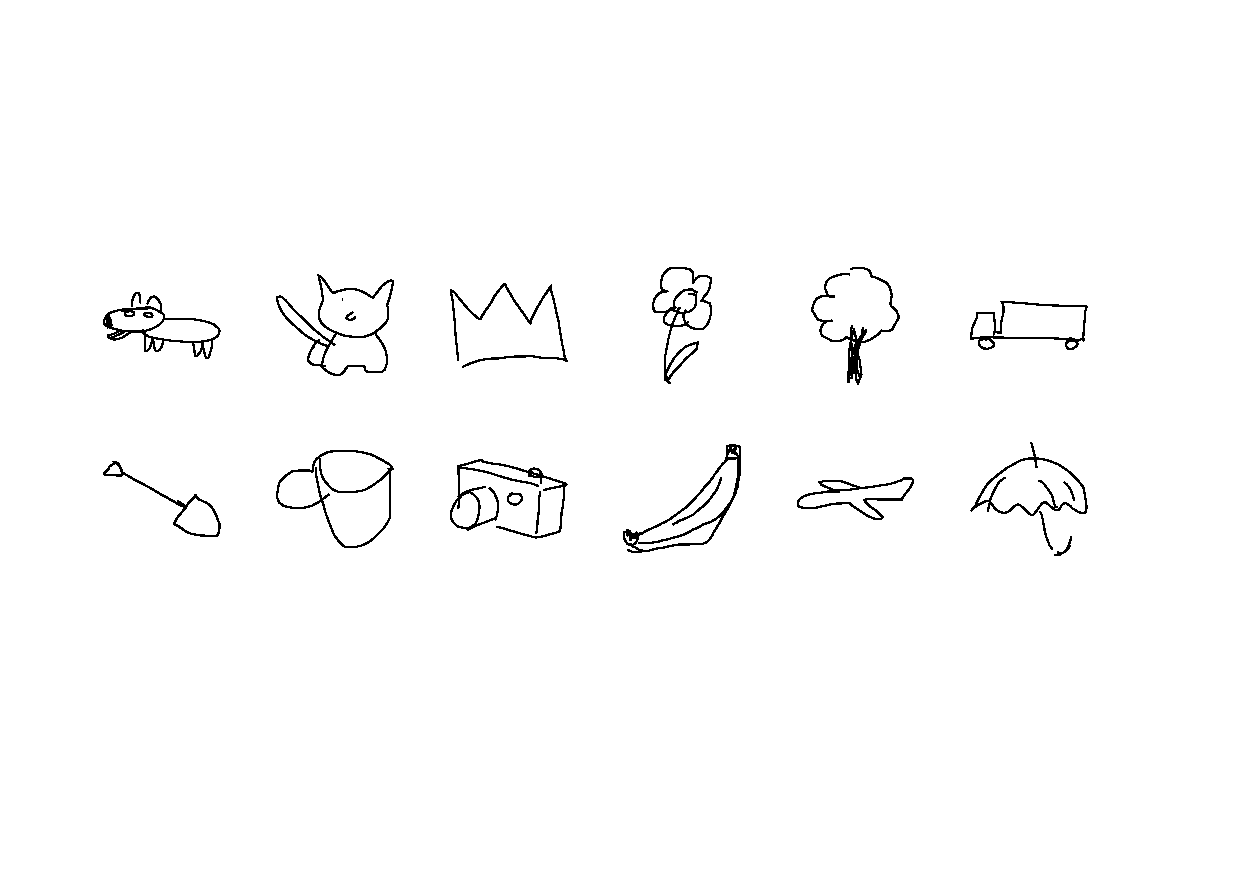
\includegraphics[width=\textwidth,trim=40 150 40 125,clip]{figures/quickdraw.pdf}
    \caption[Sample of drawings from the \emph{Quick, Draw!} dataset]{Sample of drawings from the \emph{Quick, Draw!} dataset.}
    \label{fig:quickdraw_example}
\end{figure}

\chapter{Our Approach}
\label{chap:approach}

\section{Overview}

This chapter describes the taken approach for generating images from a natural language description. In this approach, we split the task into two by generating a scene graph from the description and subsequently using the scene graph to generate the image. The image generation pipeline is depicted in \Cref{fig:pipeline} below.

\begin{figure}[h]
    \resizebox{\textwidth}{!}{
    \begin{tikzpicture}[node distance=3cm]
     
        \draw (-80bp,75bp) node[text width=7cm]{\Large \say{A duck is swimming in a pond. A tree is next to the pond.}};
    
        \draw [->] (25bp,75bp) -- (55bp,75bp);
    
        \draw (71.0bp,46.5bp) -- (71.0bp,144.5bp) -- (274.0bp,144.5bp) -- (274.0bp,46.5bp) -- cycle;
        \draw (172.5bp,133.0bp) node {\Large group};
        \draw [->] (133.19bp,92.3bp) .. controls (152.83bp,90.652bp) and (179.94bp,88.375bp)  .. (211.85bp,85.696bp);
        \draw (172.5bp,96.0bp) node {\large IN};
        \draw [->] (133.19bp,31.497bp) .. controls (153.19bp,41.417bp) and (180.93bp,55.183bp)  .. (211.85bp,70.525bp);
        \draw (172.5bp,60.0bp) node {\large NEXT TO};
        \draw (79.0bp,76.5bp) -- (79.0bp,112.5bp) -- (133.0bp,112.5bp) -- (133.0bp,76.5bp) -- cycle;
        \draw (106.0bp,94.5bp) node {\Large duck};
        \draw (212.0bp,65.5bp) -- (212.0bp,101.5bp) -- (266.0bp,101.5bp) -- (266.0bp,65.5bp) -- cycle;
        \draw (239.0bp,83.5bp) node {\Large pond};
        \draw (79.0bp,0.5bp) -- (79.0bp,36.5bp) -- (133.0bp,36.5bp) -- (133.0bp,0.5bp) -- cycle;
        \draw (106.0bp,18.5bp) node {\Large tree};
        
        \draw [->] (285bp,75bp) -- (315bp,75bp);
        
        \draw (425bp, 75bp) node{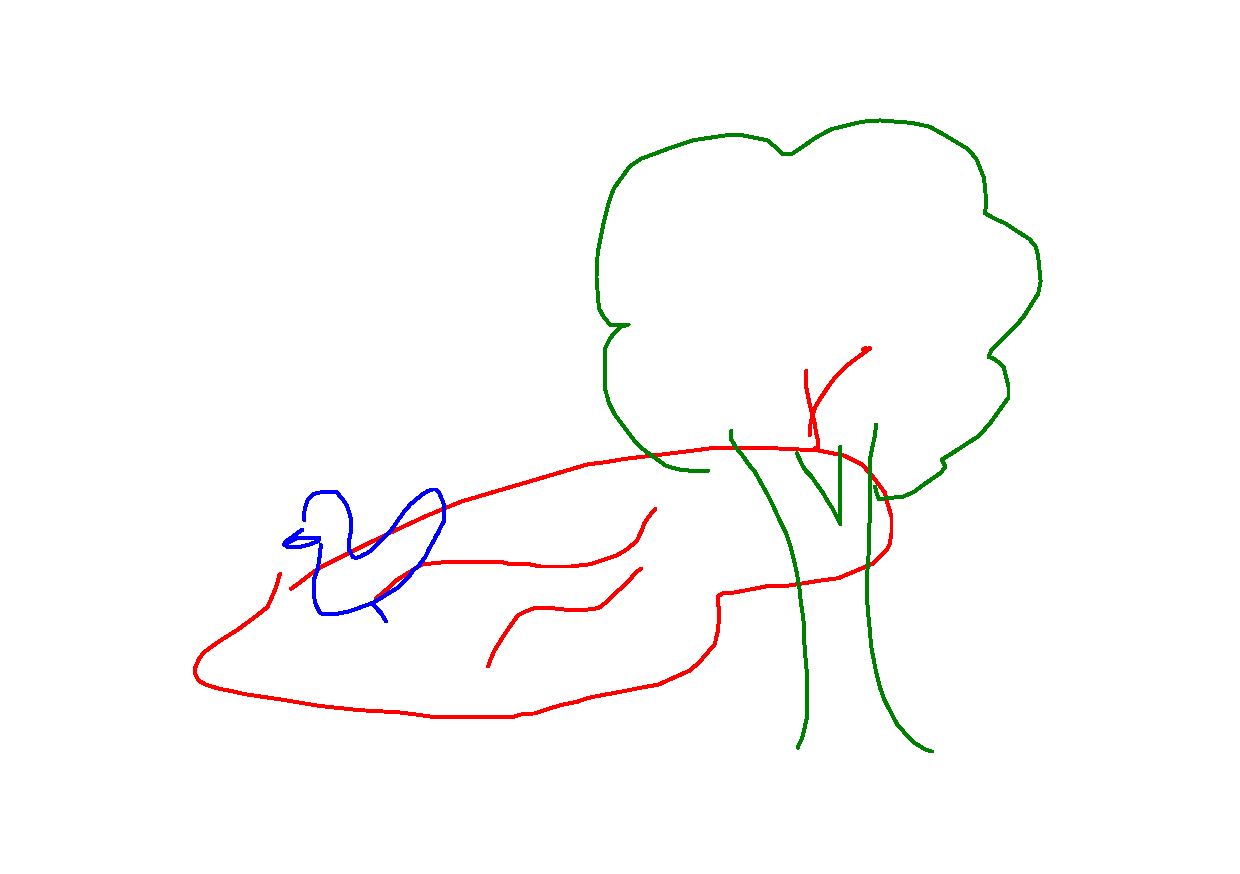
\includegraphics[width=200bp,trim=80 0 80 0,clip]{figures/duck_pond_tree_scene.pdf}};
    
    \end{tikzpicture}
    }
\end{figure}


\section{Description Processing}
\label{sec:description_processing}

The scene graph is a structure that represents the mutual relations between objects in the scene. Our approach uses syntactic analysis as a shallow semantics parser. Using syntactic analysis, we can extract relations between individual words in the sentences and use these relations to build a scene graph. In the following sections, we discuss the limitations of this approach and present a rule-based algorithm for transforming the syntactic dependency tree into a scene graph.

\subsection{Limitations}

In some cases, the syntactic structure of a sentence does not contain all the necessary semantic information to construct a corresponding scene graph. For instance, consider the two sentences \say{A man in a car is on the seat} and \say{A man in a car is on the road}. These two sentences have the same syntactic structure (\Cref{fig:dependency_trees:1}). In the first sentence, semantically, the preposition \say{on} describes the relation between the man and the seat. However, in the second sentence, the same preposition puts into relation the whole car (including the man) and the road. We do not attempt to address this problem in our thesis and accept it as a limitation of our approach.

\begin{figure}[ht]
    \centering
    \begin{subfigure}{0.4\textwidth}
        \centering
        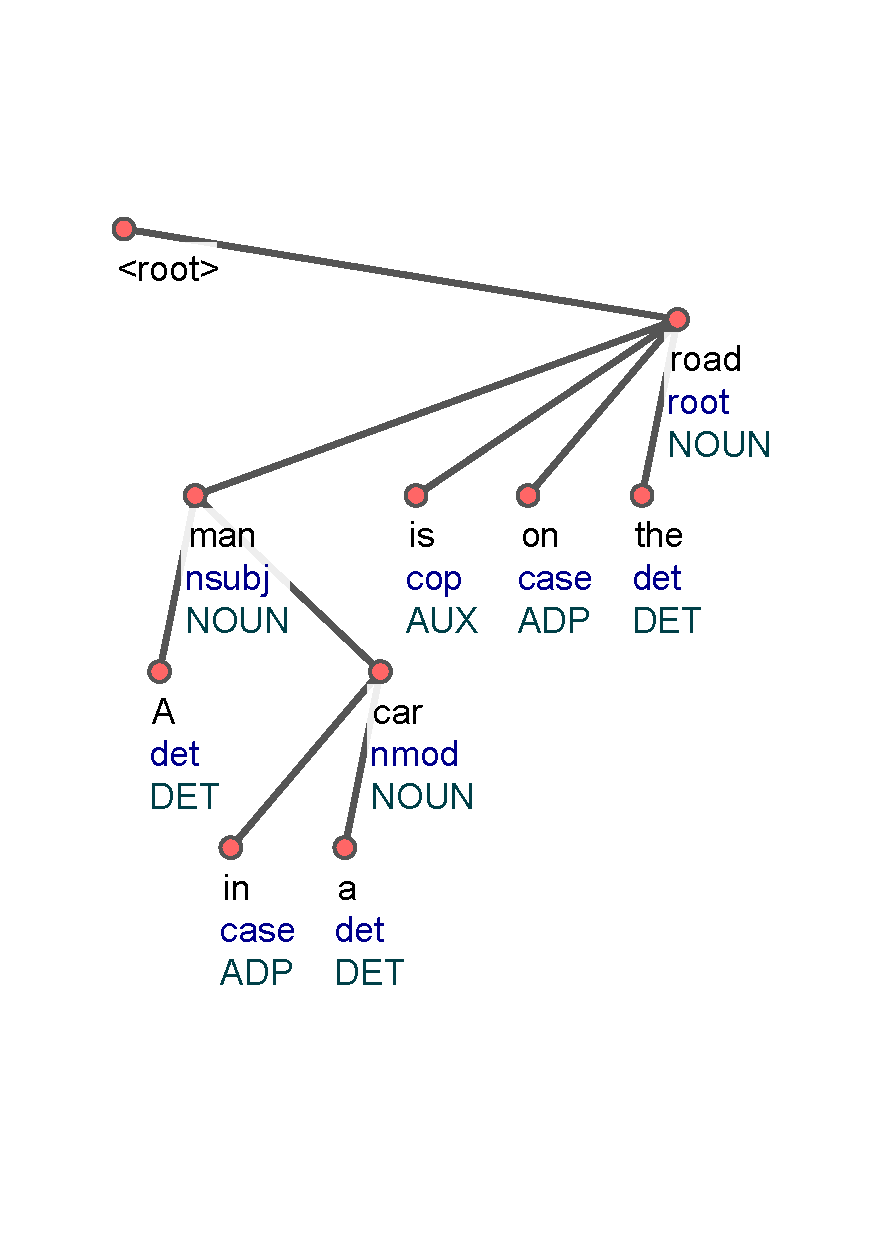
\includegraphics[width=\textwidth,trim=20 120 20 100,clip]{figures/tree_1.pdf}
    \end{subfigure}
    \hskip 25pt
    \begin{subfigure}{0.4\textwidth}
        \centering
        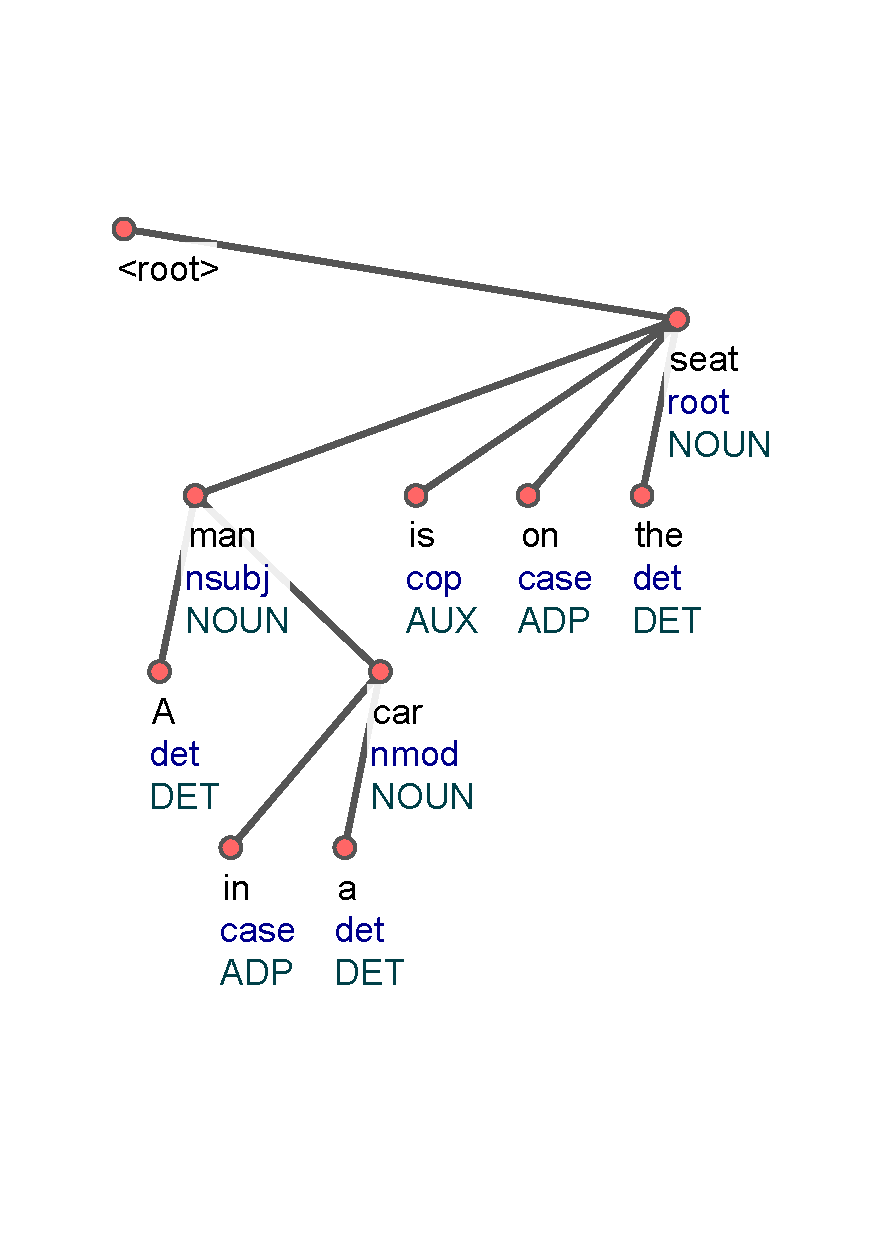
\includegraphics[width=\textwidth,trim=20 120 20 100,clip]{figures/tree_2.pdf}
    \end{subfigure}
    \caption[Sentences with the same syntactic structure but different semantics]{Sentences with the same syntactic structure but different semantics.\protect\footref{footnote:udpipe}}
    \label{fig:dependency_trees:1}
\end{figure}

\subsection{Dependency Tree Parsing}

Our approach uses a tree traversal algorithm to extract the objects and relations from the description. This algorithm is applied to a syntactic dependency tree of the description. In our implementation, we use UDPipe \citep{straka2018udpipe} to obtain the dependency trees in \emph{Universal Dependencies version 2} \citep{nivre2020universal} \emph{CoNLL-U} format. The algorithm uses some properties of this format. The implementation is further discussed in \fullref{chap:impl_details}.

\medskip

The goal of the algorithm is to identify the relations between objects in the dependency tree as semantic subject-predicate-object triples. Note that, unless stated otherwise, whenever we refer to subject-predicate-object triples, we refer to the semantic meaning, not syntactic. The algorithm searches for paths in the dependency tree that contain two nouns --- representing the subject and the object --- and an adposition representing the predicate. The algorithm can be extended to support verb predicates as well; However, we decided to restrict ourselves to position adpositions. The algorithm traverses the dependency tree in a depth-first manner, processing the nodes from left to right. While it traverses the tree, it maintains a stack of created objects. These objects are created when the algorithm opens a node with a noun. When a node with an adposition is opened, we create a new relation by taking two objects from the object stack.

\medskip

To allow relations between groups of objects, we replace the object stack with an entity stack. An entity is an abstraction of objects and groups of objects. We keep track of how many objects were created in each subtree.  If it is more than one, these objects are removed from the stack to form a group that is added to the top of the stack. Therefore, we can create a relation including a group of objects.

\medskip

Complex adpositions --- adpositions that consist of two or more words --- are concatenated into the rightmost dependency tree node. The algorithm distinguishes three complex adposition types of form: 
\begin{enumerate}
	\item adposition-adposition -- e.g. inside of
	\item adposition-noun-adposition -- e.g. in front of
    \item adverb/adjective-adposition -- e.g. next to
\end{enumerate}
A relation corresponding to the complex adposition is created in the last node; i.e., in the case of \emph{in front of} adposition, dependency tree nodes corresponding to the first two words, \emph{in} and \emph{front}, are skipped.

\medskip

Similarly, compound nouns such as paper clip, light bulb, pickup truck, and others need to be joined to create only one object. The compound nouns are identified by the \emph{Universal Dependency} \citep{nivre2020universal} relation -- \verb|compound|.

\begin{figure}[ht]
    \centering
    \begin{subfigure}{0.5\textwidth}
        \centering
        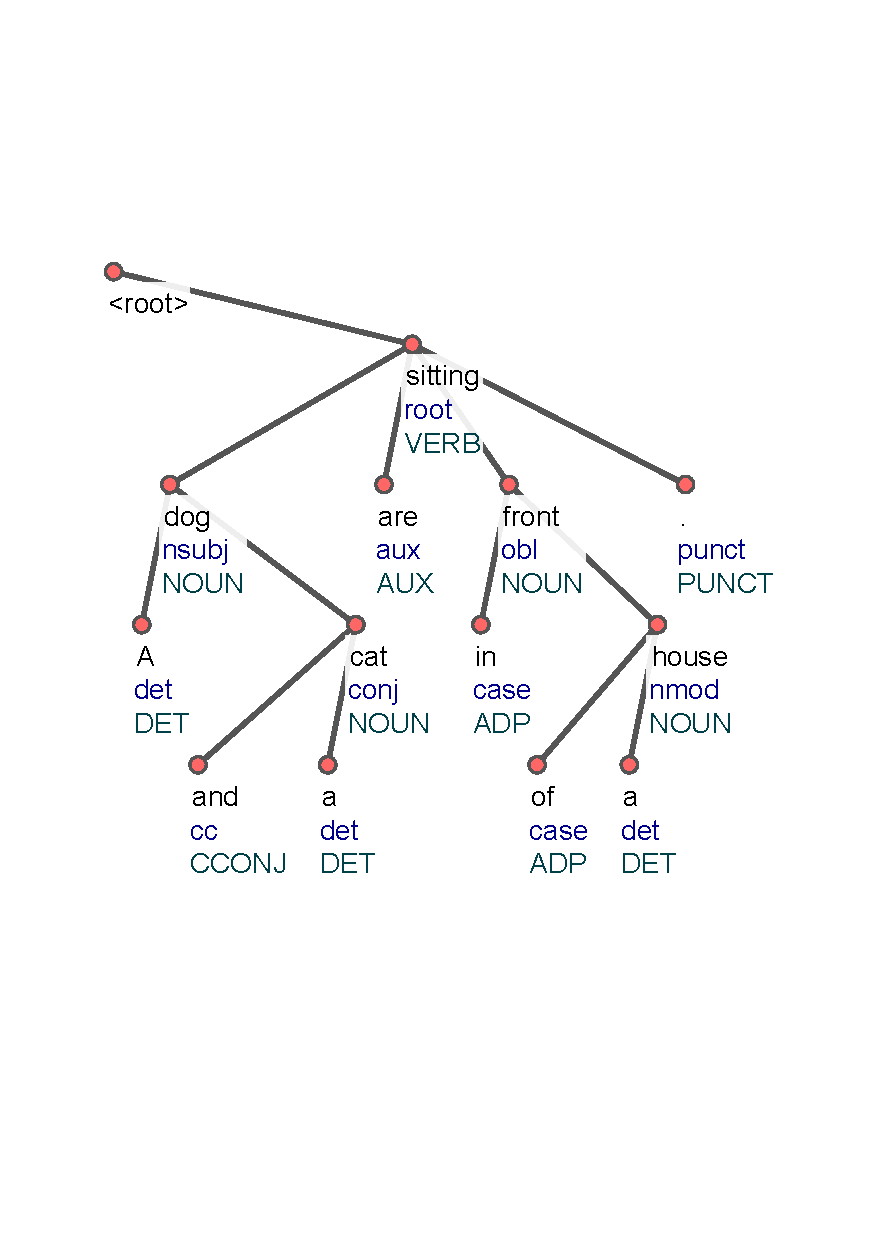
\includegraphics[width=\textwidth,trim=40 160 40 120,clip]{figures/dog_and_cat_in_front_of_house.pdf}
    \end{subfigure}
    \caption[Dependency tree of the example descripton]{Dependency tree of the example descripton.\protect\footref{footnote:udpipe}}
    \label{fig:dependency_trees:2}
\end{figure}
\addtocounter{footnote}{1}
\footnotetext{Dependency tree illustrations were generated using UDPipe LINDAT service \url{https://lindat.mff.cuni.cz/services/udpipe/}. \label{footnote:udpipe}}

\medskip

To illustrate the algorithm, consider the following description: \say{A dog and a cat are sitting in front of a house.}  \Cref{fig:dependency_trees:2} shows the syntactic tree corresponding to the description. The nodes of interest are those corresponding to words \emph{dog}, \emph{cat}, \emph{in}, \emph{front}, \emph{of}, and \emph{house}. The nodes are opened and closed by the depth-first algorithm in this order:


\begin{enumerate}
    \item open \emph{dog}
    \item open \emph{cat}
    \item close \emph{cat}
    \item close \emph{dog}
    \item open \emph{front}
    \item open \emph{in}
    \item close \emph{in}
    \item open \emph{house}
    \item open \emph{of}
    \item close \emph{of}
    \item close \emph{house}
    \item close \emph{front}
\end{enumerate}

The first two steps create new objects and put them on top of the entity stack. In the third step, the node corresponding to the \emph{cat} is closed, but there are no other entities above the cat on the stack; therefore, the stack remains intact. However, when the \emph{dog} node is closed, there is one object on the stack above -- the \emph{cat}. The two objects are therefore taken from the stack merged into a group. Next, the \emph{front} node is opened, which is skipped because it is a part of a complex adposition. The same applies for the \emph{in} node. Opening the \emph{house} node adds a new object to the entity stack. The stack now contains two entities -- The group and the house on top. In the next step, the node \emph{of} is opened. This word is the last part of the complex adposition \emph{in front of} which means that a new relation is created. A relation between the \emph{house} and the group of two objects -- the \emph{dog} and the \emph{cat}.

\section{Composing a Scene}
\label{sec:composing_scene}

The next step in our approach is composing a scene from the scene graph. The scene graph can be viewed as a set of constraints on objects and their positions in the scene. We will use the term \emph{scene composition} as a process of determining the size and position of each object in the scene. Methods used for composing a scene that satisfies the constraints are presented later in this section.

\subsection{Scene Graph Notation}
\label{sec:scene_graph_notation}

A scene graph is a directed graph with labelled edges which describes a particular scene. Each vertex corresponds to an object in the scene. Edges and their labels represent relations between the objects. Throughout this chapter, we will use the following notation for the relation "object $a$ is in relation $p$ with object $b$":
\begin{align}
    a \xrightarrow{p} b
\end{align}
For instance, $dog \xrightarrow{under} tree$ or $book \xrightarrow{on} table$. We will also refer to $a$, $b$, and $p$ as subject, object, and predicate, respectively.

\subsection{Determining the Object's Position}

To compose a scene, we need to determine where to put each object. Object positions have to satisfy the constraints given by the scene graph. In this section, we attempt to formally define the constraints and propose methods for creating and satisfying these constraints. 

\subsection{Positional Constraints}
\label{sec:constraints}

We can think of the object positions as $x$ and $y$ coordinates on a canvas. Thus, we can define the positional constraints as a function of points in the two-dimensional plane with two possible outcomes: $1$ if the constraint is satisfied and $0$ if it is not satisfied. We will denote a constraint function corresponding to a relation $a \xrightarrow{p} b$ as $C_{a,b}^p$. The constraint function is then defined as: 
\begin{align}
    C_{a,b}^p\colon \mathbb{R}^2 \rightarrow \{0, 1\}
    \label{constraint_function}
\end{align}

Suppose we have a constraint function for each relation in the scene graph. Placing an object $a$ within a scene means finding point $(x_a, y_a)$ such that \Cref{math:satisfied} holds for every object $b_i$ which is in relation $a \xrightarrow{p_i} b_i$.
\begin{align}
\label{math:satisfied}
C_{a,b_i}^{p_i}(x_a, y_a) = 1
\end{align}
However, such a point may not exist. Its existence depends on the constraint functions. Therefore, we may accept positions that satisfy a certain portion of the constraints, not necessarily all of them. The approach described in this thesis uses a Monte Carlo algorithm to find a point that satisfies the most constraints on an object. 

\medskip

The Monte Carlo algorithm generates $N$ random normally distributed points $(x_0, y_0), \dots , (x_N, y_N); x_i \sim \mathcal{N}(x_b, w_b), y_i \sim \mathcal{N}(y_b, h_b)$ where $(x_b, y_b)$ and $(w_b, h_b)$ denote the centre of the object and size of object $b$ respectively. Each of the points is tested using all constraint functions associated with objects $a$ and $b$. The first point that satisfies the largest number of constraints is designated as the position of object $a$. This algorithm requires prior knowledge of the position of object b, which requires the existence of topological ordering of the scene graph. 

\subsection{Rule-Based Constraints}
\label{sec:rule_based_constraints}

In the first approach, we define 5 elementary constraint functions and combine these functions to define constraints for selected adpositions. The five constraint functions are:
\begin{enumerate}
    \item \emph{On} constraint -- Tests whether a point is near the top of the object to which the constraint relates. 
    \item \emph{Side} constraint -- Defines a half-plane; all points in the half-plane satisfy the constraint.
    \item \emph{Box} constraint -- Tests whether a point lies within a box.
    \item \emph{Inside} constraint -- Treats the object it relates to as a polygon. A point satisfies this constraint if it lies inside the polygon.
    \item \emph{Disjunction} constraint -- A composite constraint that encapsulates two or more other constraints. The constraint is satisfied if at least one of the encapsulated constraints is satisfied.
\end{enumerate}

\begin{table}[ht]
    \small
    \centering
    \begin{threeparttable}
        \begin{tabular}{p{0.2\linewidth}|p{0.7\linewidth}}
            \textbf{Adposition} & \textbf{Elementary constraint} \\
            \hline \hline
            \emph{in}       &  \emph{Inside} constraint \\
            \hline
            \emph{inside}    & \emph{Inside} constraint \\
            \hline
            \emph{inside of} & \emph{Inside} constraint \\
            \hline
            \emph{on}        & \emph{On} constraint \\
            \hline
            \emph{under}     & \emph{Side} constraint \\
            \hline
            \emph{below}     & \emph{Side} constraint \\
            \hline
            \emph{above}    & \emph{Side} constraint \\
            \hline
            \emph{behind}    & \emph{Box} constraint \\
            \hline
            \emph{in front of} & \emph{Box} constraint \\
            \hline
            \emph{next to} & \emph{Disjuction} constraint (containing two \emph{side} constraints)
        \end{tabular}
    \end{threeparttable}
    \caption[Rule-based constraints]{Rule-based constraints.}
    \label{tab:rule_based_constraints}
\end{table}

Using these elementary constraints we define constraint functions for a small set of adpositions -- \emph{in}, \emph{inside}, \emph{inside of}, \emph{on}, \emph{under}, \emph{below}, \emph{above}, \emph{behind}, \emph{in front of}, and \emph{next to}. \Cref{tab:rule_based_constraints} shows which elementary constraints are used to define the constraints for the listed adpositions. \Cref{sec:constraints_impl} describes how each of the elementary constraints is implemented and provides details on how are these constraints combined. 

\begin{figure}[ht]
    \centering
    \begin{subfigure}{0.45\textwidth}
        \centering
        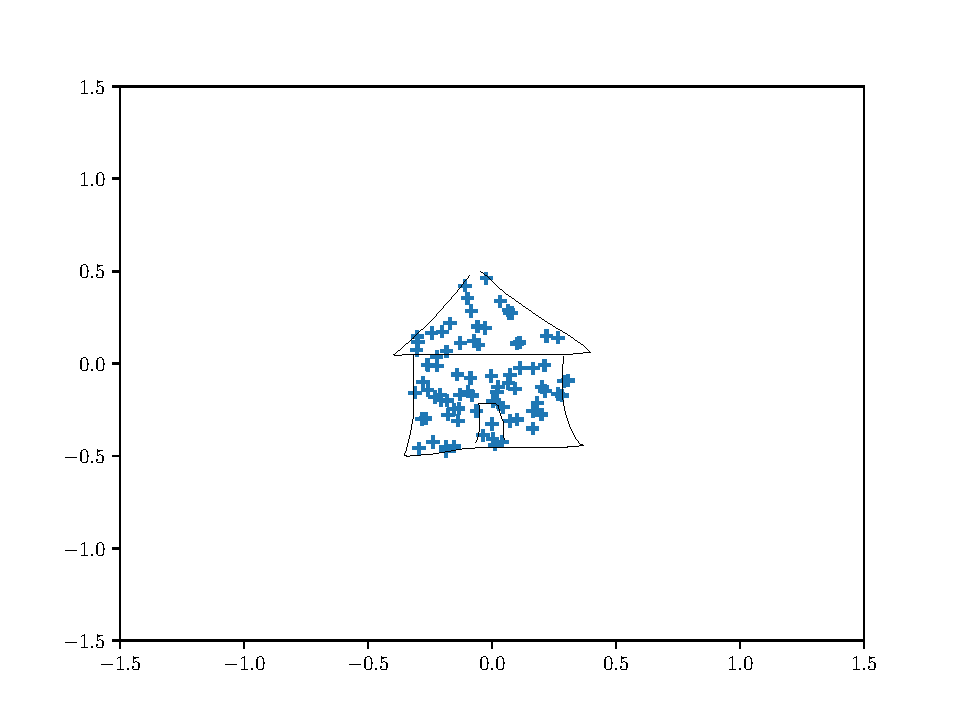
\includegraphics[width=\textwidth]{figures/rule_in_house.pdf}
    \end{subfigure}
    \begin{subfigure}{0.45\textwidth}
        \centering
        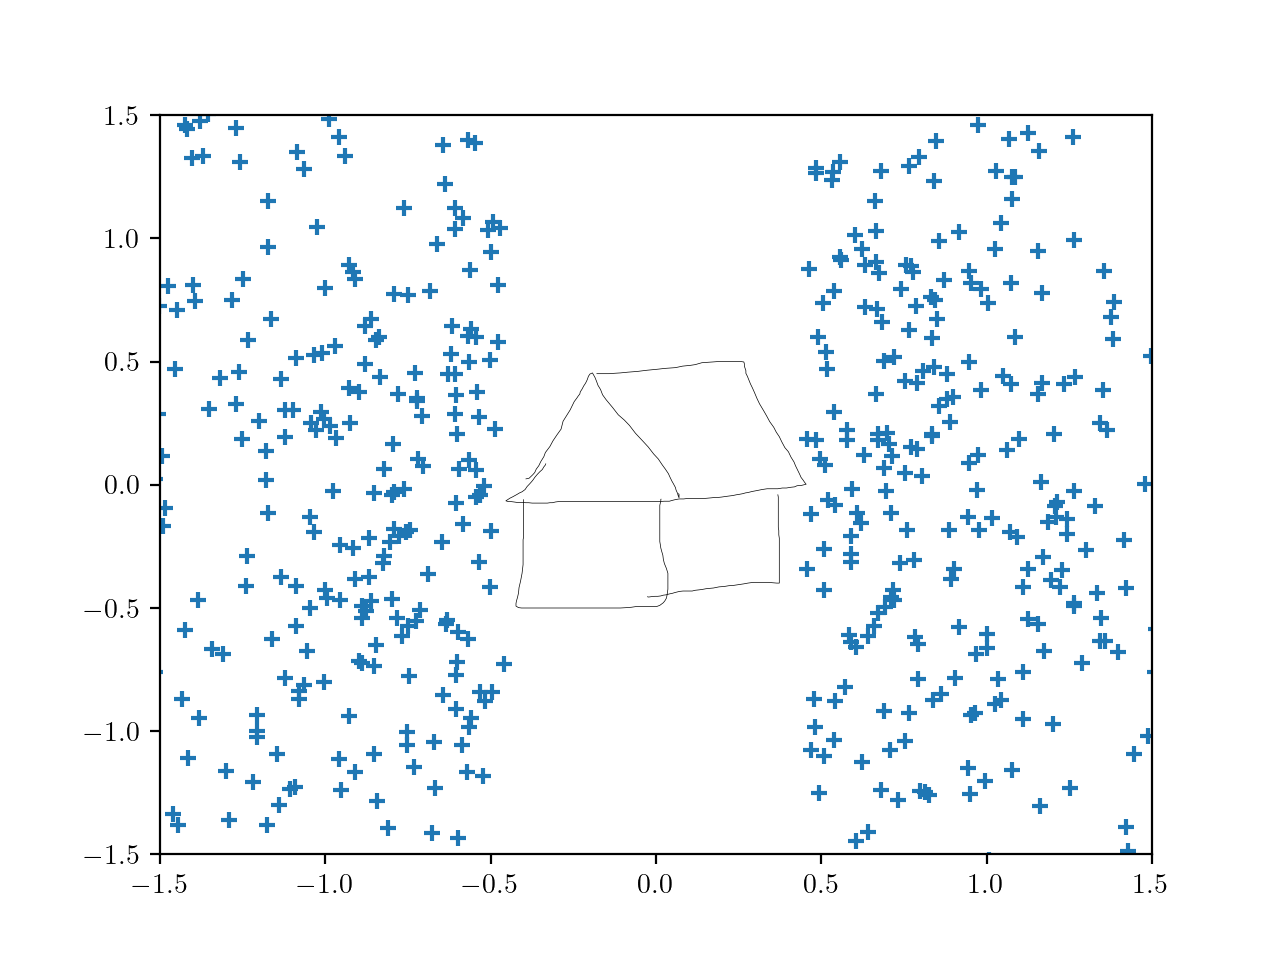
\includegraphics[width=\textwidth]{figures/rule_disjunct_side_house.png}
    \end{subfigure}
    \caption[Monte Carlo algorithm with rule-based constraints]{Monte Carlo algorithm finds points that satisfy given constraints. \emph{Inside} constraint on the left, \emph{side} constraint on the right.}
    \label{fig:monte_carlo:1}
\end{figure}

\subsection{Classifier-Based Constraints}
\label{sec:classifier_based_constraints}

The other approach uses a binary classifier trained on the \emph{Scene Graph} \citep{xu2017scenegraph}\break dataset. The classifier matches the constraint function definition \ref{constraint_function}. Given coordinates $(x, y)$, subject $a$, object $b$, and predicate $p$, the classifier decides whether the coordinates $(x, y)$ satisfy the constraint given by $a \xrightarrow{p} b$.

\begin{figure}[ht]
    \centering
    \begin{subfigure}{0.45\textwidth}
        \centering
        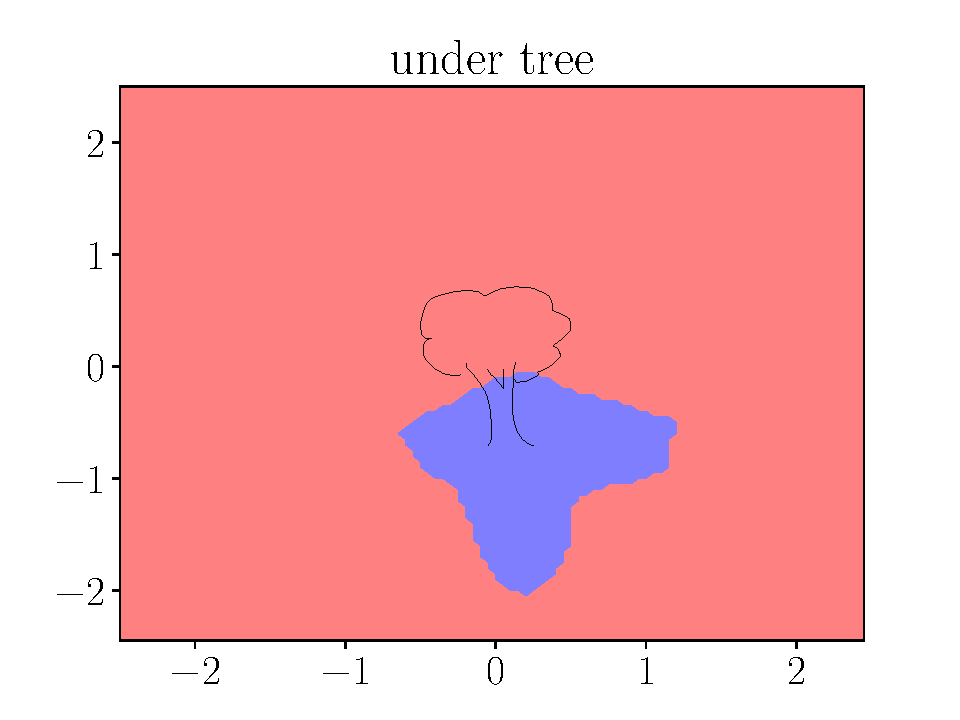
\includegraphics[width=\textwidth]{figures/under_tree}
    \end{subfigure}
    \begin{subfigure}{0.45\textwidth}
        \centering
        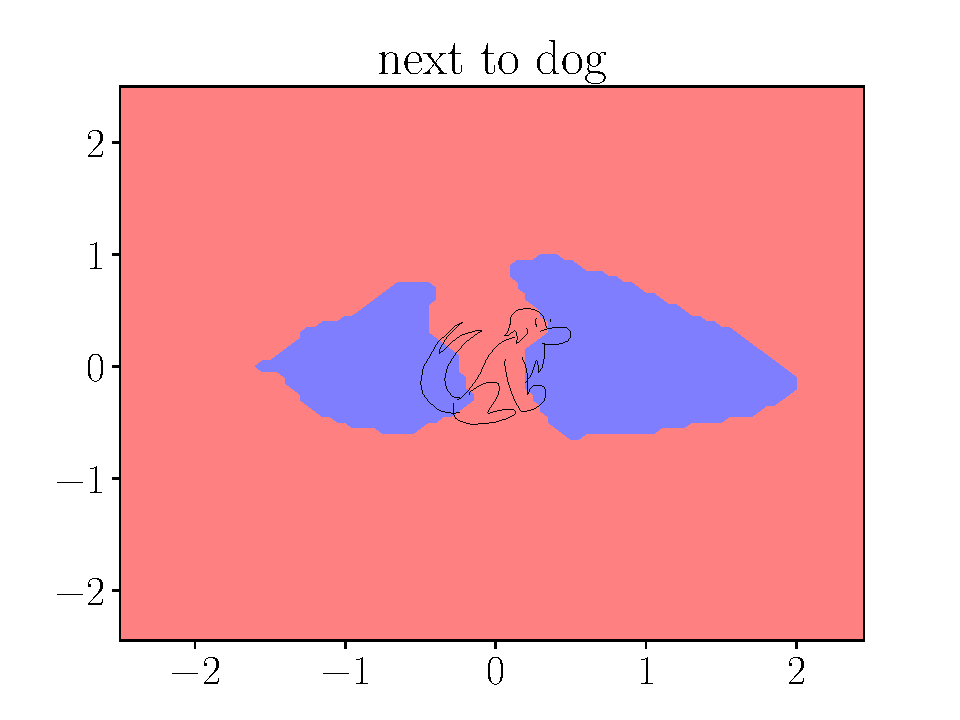
\includegraphics[width=\textwidth]{figures/next_to_dog}
    \end{subfigure}
    \caption[Visualisation of the classifier's decision boundaries]{Visualisation of the classifier's decision boundaries.}
    \label{fig:boundaries:1}
\end{figure}

\medskip

The classifier has four inputs -- subject, predicate, $x$ coordinate, and $y$ coordinate. The subject is encoded as a 100-dimensional vector using word embedding. The \emph{Scene Graph} dataset \citep{xu2017scenegraph} contains a limited number of predicates. We use the 50 most frequent ones; therefore, the predicate is encoded using a 50-dimensional one-hot vector. Each of the $x$ and $y$ coordinates is encoded as a single float number. Note that we use normalised coordinates relative to the centre of the subject -- the absolute $x$ and $y$ coordinates are converted to relative ones and divided by subjects' width and height, respectively.  In total, the classifier takes a 152-dimensional input. In \Cref{sec:constraint_results}, we also show results obtained with a classifier that only takes the predicates and the coordinates as inputs.

\medskip

The classifier itself is a multilayer perceptron with three hidden layers and a total of $600$ hidden units with ReLU activations. We use Stochastic Gradient Descent (SGD) as an optimiser and a cross-entropy loss.

\medskip

The source of the training data is the \emph{Scene Graph} dataset \citep{xu2017scenegraph}. The dataset contains the semantic subject-predicate-object triples as well as sizes and positions of the subjects and objects. The positions are absolute. We convert them to the relative position format described in the preceding sections. However, this dataset only contains correctly placed objects. To be able to train the classifier, we need to synthesise data that contains incorrectly placed objects. We do so by replacing the relative position of a subject-object-predicate triple with a position of another triple with a different predicate.

\subsection{Determining the Object's Size}
\label{sec:determining_obj_size}

Besides the object positions within a scene, we also need to determine their sizes. The \emph{Quick, Draw!} \citep{quickdraw} dataset contains $345$ categories. The relatively small number of categories makes it possible to define the absolute size for each category by hand. This is, in fact, our first approach for determining the object sizes. The objects in the scene can be scaled accordingly to the ratio between the defined sizes. In addition to the process being tedious, this approach also has one apparent flaw. The size ratio of objects often depends on context. For instance, the size ratio of a television and a car is different in the following sentences: \say{A car is on the television} and \say{The television is near the car.}.

\medskip

The mentioned problem of absolute sizes suggests a different approach. Instead of defining the absolute size for each category, we can define a relative size between a pair of categories. However, defining relative sizes for $119\,025$ pairs of categories by hand is infeasible. Instead, we once again use the \emph{Scene Graph} \citep{xu2017scenegraph} dataset to extract the relative sizes. The following list summarizes three methods used to determine the objects' sizes:
\begin{enumerate}
    \item Absolute -- For each \emph{Quick, Draw!} category, we extract absolute sizes of matching objects' bounding boxes from the dataset and use their average as a size.
    \item Relative -- If both subject and object are valid \emph{Quick, Draw!} categories, we compute the ratio of their widths and heights. We average these ratios across the whole dataset.
    \item Relative + word embedding -- Modification of the previous method where we do not require an exact match with a \emph{Quick, Draw!} category. Instead, we add the ratios to the most similar categories. The most similar categories are determined by the cosine similarity of their word embeddings. We also set different similarity thresholds. 
\end{enumerate}

Not all the \emph{Quick, Draw!} category pairs are present in the \emph{Scene Graph} dataset. To address this problem, the data obtained using the methods mentioned above can be completed by transitive closure. We estimate the unknown ratio $a:b$ between objects $a$ and $b$ as 
\begin{align*}
\frac{a}{b} = \frac{1}{n} \sum_{i = 0}^n \frac{a}{k_i} \cdot \frac{k_i}{b}
\end{align*}
where $a:k_i$ and $k_i:b$ are known ratios.

\section{Image Generation}

With a composed scene, the image generation itself is a straightforward process. Both position and size are known for all objects in the scene. The only thing left to do is to select a drawing of the object and draw it onto a drawing canvas. The drawings are randomly selected from the \emph{Quick, Draw!} \citep{quickdraw} dataset. We do not use the entire dataset as it also contains irrelevant and inappropriate data. Only a manually selected portion of the dataset is used.

\chapter{Implementation Details}
\label{chap:impl_details}

This chapter provides details about the implementation of the approach proposed in \Cref{chap:approach}. The implementation is written in Python 3. Its source code can be found in \Cref{attachment:sources}.

\section{Overview}

The implementation consists of three main components: a description processor, a scene composer, and a renderer. These components are depicted in \Cref{fig:impl_diagram}. The components and transitions between the components correspond to the drawing generation pipeline presented in \Cref{chap:approach}.
\begin{figure}[h]
    \centering
    \begin{tikzpicture}[node distance=3cm]
        \tikzstyle{box} = [draw, thick, rectangle, minimum height=1.25cm, minimum width=4.5cm];
        \tikzstyle{smallerbox} = [draw, thick, rectangle, minimum height=1cm, minimum width=3.5cm];
    
        \clip (-3cm,-1cm) rectangle + (12cm,-9cm);

        \node(empty){};
        \node(descproc)[box, below of=empty]{Description Processor};
        \node(scenecomp)[box, below of=descproc]{Scene Composer};
        \node(renderer)[box, below of=scenecomp]{Renderer};

        \node(objfactory)[smallerbox, right of=scenecomp, yshift=0.5cm, xshift=3cm]{Object Factory};
        \node(objscaler)[smallerbox, right of=scenecomp, yshift=-0.5cm, xshift=3cm]{Object Scaler};

        \draw [->, thick] ++(0, -1cm) -- node[draw, fill=white, draw=none]{\small Description} (descproc);
        \draw [->, thick] (descproc) -- node[draw, fill=white, draw=none]{\small Scene Graph} (scenecomp);
        \draw [->, thick] (scenecomp) -- node[draw, fill=white, draw=none]{\small Drawing Representation} (renderer);
        \draw [<->, thick] (scenecomp.east) -- ++(1cm, 0) |- (objfactory);
        \draw [<->, thick] (scenecomp.east) -- ++(1cm, 0) |- (objscaler);
    \end{tikzpicture}
    \caption[Implementation diagram]{Implementation diagram.}
    \label{fig:impl_diagram}
\end{figure}

Besides the three main components, the diagram in \Cref{fig:impl_diagram} also contains two other components: an object factory and an object scaler. Together with the scene composer component, these two components implement the algorithms proposed in \fullref{sec:composing_scene}. Each of the components is discussed in more detail in the following sections.

\section{Description Processor}

The description processor is a component responsible for converting the input text into a scene graph. Description processor has one public method \verb|process|. The method has the following Python signature: 
\begin{verbatim}
process(self, text: str) -> Scene
\end{verbatim}

\Cref{attachment:sources} contains one implementation of the description processor - \break \verb|UDPipeDescriptionProcessor|. This implementation uses UDPipe \citep{straka2018udpipe} for syntactic analysis. The dependency tree traversal algorithm was described in the \fullref{sec:description_processing}. The \verb|resources/predicates| file contains a list of allowed predicates which can be processed by the processor.

\medskip

The \verb|Scene| class represents a scene graph. It contains two types of entities: \verb|Object| and \verb|Group| entities (subclasses of \verb|Entity|). Each entity has a list of relations represented by \verb|Relation|. 

\medskip

The \verb|Group| entity is just a convenience class which encapsulates other entities. Every group's relation is redirected to each entity within the group. We can extend the notation introduced in \fullref{sec:scene_graph_notation}, such that $[a, b]$ will denote a group of objects $a$ and $b$. Then $[a, b] \xrightarrow{p} c$ will effectively become $a \xrightarrow{p} c$ and $b \xrightarrow{p} c$. Similarly $a \xrightarrow{p} [b, c]$ will become $a \xrightarrow{p} c$ and $a \xrightarrow{p} c$.

\medskip

Apart from the relations, the \verb|Object| class also contains the attribute \verb|word|. This attribute holds a noun that describes the object. Note that in the case of composite nouns, this attribute may contain multiple words. 

\section{Scene Composer}

The scene composer determines the position of every object in the scene. The scene composer is a class with the following method:
\begin{verbatim}
compose(self, scene: Scene) -> List[PhysicalObject]
\end{verbatim}

\medskip

\verb|ConstraintComposer| is an implementation of the algorithm described in \fullref{sec:constraints}. The \verb|ConstraintComposer| associates each object in the scene with a corresponding \verb|Constraint| object. Then it uses these constraints to determine the positions using the described Monte Carlo algorithm. 

\medskip

The \verb|Constraint| is an abstract callable class. As opposed to the constraint function defined in \fullref{sec:constraints}, the \verb|Constraint| object operates on a batch of coordinates. It returns a Boolean array that masks the coordinates which satisfy the constraint. Using the notation from Section \ref{sec:scene_graph_notation}, we can describe the Python \verb|Constraint| call method:
\begin{verbatim}
__call__(self, xs: np.ndarray, ys: np.ndarray) -> np.ndarray
\end{verbatim}
As a mapping between two vectors:
\begin{align}
[(x_0, y_0), \ldots, (x_n, y_n)] \mapsto [C_{a,b}^p(x_0, y_0), \ldots, C_{a,b}^p(x_n, y_n)]
\end{align}

The scene composer generates a single set of random coordinates for one object. These coordinates are applied to every constraint associated with the object. The resulting boolean arrays are summed as integer arrays. By applying $argmax$ to this array, we find an index of coordinates that satisfy most of the constraints. These coordinates are used as the object's position. In other words, for a fixed object $a$, we set its position to be $(x_i, y_i)$, where:
\begin{align}
i = \argmax \sum_{(b, p)} [C_{a,b}^p(x_0, y_0), \ldots, C_{a,b}^p(x_n, y_n)]
\end{align}

\subsection{Constraints}
\label{sec:constraints_impl}

\Cref{sec:rule_based_constraints} lists a set of elementary constraints. In this section, we take a closer look at these constraints, describe how they are implemented and how they are combined to define constraints for specific adpositions. All constraints are implemented as subclasses of \verb|Constraint| which was described in the previous section. The constraints are initialised with an object and predicate that relates to the object. Information about the object and predicate are used to determine whether a point in plane satisfies the constraint.

\medskip

The \verb|OnConstraint| takes the upper $25\%$ of the object's drawing strokes. The constraint tests if a point is within a certain distance from these strokes. The distance is specified by attribute \verb|limit|.

\medskip

The \verb|SideConstraint| defines a half-plane. All points in this half-plane satisfy the constraint.  The constraint has two attributes -- \verb|direction| and \verb|offset|. The \verb|direction| attribute is a vector normal to the half-plane boundary.  The \verb|offset| attribute moves the boundary further away from the object.

\medskip

The \verb|BoxConstraint| is satisfied whenever a point lies inside a bounding box of the object to which the constraint relates. In addition, the implementation also contains an attribute \verb|scale| that can scale the bounding box up or down.

\medskip

The \verb|InsideConstraint| tests whether a point lies within an area spanned by the object it relates to. The area is given by strokes of drawing associated with the object. We consider each stroke to be a polygon. We test whether a point lies inside a polygon defined by one of the strokes. Some strokes contain many line segments, which could lead to a slow evaluation of the constraint. Hence, we apply the Ramer-Douglas-Peucker \citep{douglas1973algorithms} algorithm to the drawing to reduce its number of line segments.

\medskip

The primary purpose of \verb|DisjunctionConstraint| is to combine other non-overlapping constraints. The constraint is satisfied when any of the constraints it encapsulates is satisfied. Since we assume the encapsulated constraints are non-overlapping, only one of the constraints can be satisfied at a time. The same could be achieved by specifying more constraints for a single predicate. However, using the disjunction constraint does not require evaluating all the constraints~-- the evaluation ends after the first satisfied constraint. The non-overlapping regions can be seen in the right image of \Cref{fig:monte_carlo:1}. 

\medskip

\Cref{tab:rule_based_constraints_impl} below shows how the elementary constraints are used in the rule-based approach to form constraint functions for adpositions listed in \Cref{sec:rule_based_constraints}.

\begin{table}[ht]
    \small
    \centering
    \begin{threeparttable}
        \begin{tabular}{p{0.2\linewidth}|p{0.7\linewidth}}
            \textbf{Adposition} & \textbf{Elementary constraint} \\
            \hline \hline
            \emph{in}        &  \verb|InsideConstraint()| \\
            \hline
            \emph{inside}    & \verb|InsideConstraint()| \\
            \hline
            \emph{inside of} & \verb|InsideConstraint()| \\
            \hline
            \emph{on}        & \verb|OnConstraint()| \\
            \hline
            \emph{under}    & \verb|SideConstraint(direction=(0, 1))| \\
            \hline
            \emph{below}    & \verb|SideConstraint(direction=(0, 1))| \\
            \hline
            \emph{above}     & \verb|SideConstraint(direction=(0, -1))| \\
            \hline
            \emph{behind}    & \verb|BoxConstraint()| \\
            \hline
            \emph{in front of} & \verb|BoxConstraint()| \\
            \hline
            \emph{next to} & \begin{minipage}[t]{\linewidth}
            \begin{verbatim}
DisjunctionConstraint([
    SideConstraint(direction=(-1, 0)),
    SideConstraint(direction=(1, 0))
])\end{verbatim}
            \end{minipage}\vspace{4pt} \\
            \hline
            unknown & \begin{minipage}[t]{\linewidth}
            \begin{verbatim}
DisjunctionConstraint([
    SideConstraint(direction=(-1, 0)),
    SideConstraint(direction=(1, 0)),
    SideConstraint(direction=(0, 1)),
    SideConstraint(direction=(0, -1)),
])\end{verbatim}
            \end{minipage}\vspace{4pt}
        \end{tabular}
        \begin{tablenotes}
            \small
            \item Some constructor arguments are omitted for brevity.
        \end{tablenotes}
    \end{threeparttable}
    \caption[Rule-based constraints implementation]{Rule-based constraints implementation.}
    \label{tab:rule_based_constraints_impl}
\end{table}

\verb|ClassifierConstraint| implements the classfier-based approach described in \fullref{sec:classifier_based_constraints}. The classifier uses \emph{scikit-learn's} \citep{scikit-learn} multi-layered perceptron classifier trained on the \emph{Scene Graph} dataset. The trained model is loaded from \verb|resources/sklearn/constraints.model| file. All relevant details about the model are discussed in \Cref{sec:classifier_based_constraints}.

\subsection{Object Factory}

The object factory is a class with a method with the following Python signature:
\begin{verbatim}
get_physical_object(self, obj: Object) -> PhysicalObject
\end{verbatim}

\verb|QuickDrawObjectFactory| instantiates a \verb|PhysicalObject| using Quick, Draw! \citep{quickdraw} Data. It uses a \verb|WordEmbedding| class for resolving objects which are not present in the \emph{Quick, Draw!} categories.

\medskip

\verb|WordEmbedding| class is a wrapper around a \emph{fasttext}  \citep{bojanowski2017enriching} model. It has a single method \verb|most_similar_word(self, word: 'str') -> 'str'| which finds the most similar word from a list of words based on the cosine similarity. The list of words is, in this case, a list of \emph{Quick, Draw!} categories.

\subsection{Object Scaler}

The object scaler determines the object sizes. The object scaler class has the following Python signature:

\begin{verbatim}
scale(self, sub: PhysicalObject, obj: PhysicalObject, 
            pred: str) -> float
\end{verbatim}

This method scales the subject \verb|sub|. The size estimation may use the context given by the object \verb|obj| or the predicate \verb|pred|. The size estimation strategy depends on the implementation. We provide two object scaler implementations~--~\verb|AbsoluteObjectScaler| and \verb|RelativeObjectScaler|. These clases implement the object scaling methods described in \fullref{sec:determining_obj_size}.

\medskip

The \verb|AbsoluteObjectScaler| scales the \verb|sub| object according to a table of absolute (hand crafted) sizes located in \verb|resources/quickdraw/attributes.csv|. The file contains a width and/or height for the given \emph{Quick, Draw!} category.

\medskip

The \verb|RelativeObjectScaler| takes into account both subject and object (\verb|sub| and \verb|obj|). The subject is scaled according to a table of relative sizes located in \verb|resources/quickdraw/attributes_relative.csv| file. The file contains width and height ratios for the given pair of \emph{Quick, Draw!} categories. The size of \verb|obj| has to be known before calling the \verb|scale| method. Its size is multiplied by the ratio specified in the file to determine the subject's size.

\section{Renderer}

The renderer is the last component in the system. The only purpose of the renderer is to render a final drawing from a \verb|PhysicalObject| list. Two different renderers are provided. The first one, \verb|SimpleRenderer|, renders a PNG image. This renderer is used in the command-line interface. The other renderer has a form of a web application written in JavaScript. The composed scene served over HTTP is rendered onto an HTML canvas. The web interface is discussed in more detail in \fullref{sec:web_interface}.

\chapter{User Manual}

\section{Prerequisites}

Make sure that the following are installed on your system before proceeding to the installation:

\begin{itemize}
    \item GNU Make
    \item Python 3
\end{itemize}

\section{Installation}

All Python dependencies and required pre-trained models can be downloaded and installed by running the following command in \verb|drawtomat/| directory:

\begin{verbatim}
    make install
\end{verbatim}

\section{Command-Line Interface}

The command-line interface can be started by
\begin{verbatim}
    make run
\end{verbatim}
or alternatively:

\begin{verbatim}
    export PYTHONPATH=src
    python3 -m drawtomat [-h] [--help]
                         [--description DRAWING_DESCRIPTION] 
                         [--graph_output GRAPH_OUTPUT_PATH]
                         [--image_output IMAGE_OUTPUT_PATH]
                         [--sizes {absolute,relative}]
                         [--constraints {rule,classifier}]
                         [--show]
\end{verbatim}

If the \verb|--description| flag is not set, the program takes the description from the standard input. A path to a generated drawing can be set by \verb|image_output|. The default is \verb|./drawing.png|. If the \verb|--show| flag is set, the image is opened immediately after it is generated. If the \verb|--graph_output| flag is set, a scene graph will be saved to the specified file in the Graphviz DOT language. Note that when running the program without Make, one needs to activate the Python virtual environment beforehand. Options \verb|sizes| and \verb|constraints| allows user to choose the approach for determining object size and position.

\section{Web Interface}
\label{sec:web_interface}

\subsection{Server}

The implementation contains a Flask web server, which provides a simple HTTP API. The server can be started by running the following command:

\begin{verbatim}
    make run-api
\end{verbatim}

The API has a single endpoint \verb|POST /drawtomat|. The format of request and response bodies are described by tables \ref{tab:api_request} and \ref{tab:api_response}. Both tables specify JSON formats accepted and provided by the API.

\begin{table}[ht]
    \small
    \centering
    \begin{tabular}{p{0.3\linewidth}|p{0.1\linewidth}|p{0.5\linewidth}}
        \textbf{Key} & \textbf{Type} & \textbf{Description} \\
        \hline \hline
        \verb|description| & \verb|string| & A description of a drawing (limited to $1000$ characters). \\
        \hline
        \verb|options| & \verb|object| & Drawing generation options. \\
        \hline
        \verb|options.constraints| & \verb|string| & Allowed values are \verb|absolute| or \verb|relative|. If the value is equal to \verb|"classifier"|, positions of objects in the scene will be determined using the classifier-based approach. \\
        \hline
        \verb|options.sizes| & \verb|string| & Allowed values are \verb|"rule"| or \verb|"classifier"|. If the value is equal to \verb|"relative"|, sizes of objects in the scene will be determined based on size ratios extracted from \emph{Scene Graph} dataset. \\
    \end{tabular}
    \caption[Request JSON format]{Request JSON format.}
    \label{tab:api_request}
\end{table}

\begin{table}[ht]
    \small
    \centering
    \begin{tabular}{p{0.2\linewidth}|p{0.1\linewidth}|p{0.6\linewidth}}
        \textbf{Key} & \textbf{Type} & \textbf{Description} \\
        \hline \hline
        \verb|description| & \verb|string| & A description of a drawing. \\
        \hline
        \verb|bounds| & \verb|object| & Defines a bounding box of the drawing. \\
        \hline
        \verb|bounds.top| & \verb|number| & The maximum of all $y$ coordinates. \\
        \hline
        \verb|bounds.bottom| & \verb|number| & The mininum of all $y$ coordinates.  \\
        \hline
        \verb|bounds.right| & \verb|number| & The maximum of all $x$ coordinates. \\
        \hline
        \verb|bounds.left| & \verb|number| & The minimum of all $x$ coordinates. \\
        \hline
        \verb|drawing| & \verb|array| & Drawing representation similar to \emph{Quick, Draw!} format. The drawing is represented as an array of objects in the scene. Objects are arrays of strokes. Each stroke is an array itself containing three sequences - $x$ coordinates, $y$ coordinates and time in milliseconds. \\
    \end{tabular}
    \caption[Response JSON format]{Response JSON format.}
    \label{tab:api_response}
\end{table}

\subsubsection{Sample Request}
\begin{verbatim}
POST /drawtomat HTTP/1.1
Host: localhost:5000
Content-Type: application/json

{
    "description": "A dog is sitting under a tree.",
    "options": {
        "constraints": "classifier",
        "sizes": "relative"
    }
}
\end{verbatim}

\subsubsection{Sample Response}

\begin{verbatim}
HTTP/1.1 200 OK
Content-Type: application/json
Server: Werkzeug/1.0.1 Python/3.8.6
Date: Thu, 11 Mar 2021 09:37:29 GMT

{
    "bounds": {
        "bottom": 197.13186109372901,
        "left": -187.71175260273606,
        "right": -10.021259329191409,
        "top": 442.4159101648598
    },
    "description": "A dog is sitting under a tree.",
    "drawing": [
        [
            [
                [-84.61983725860478, ..., -69.03160196448714],
                [268.89656697608194, ..., 345.9553905054937],
                [0, ...,  553]
            ],
            ...
        ]
    ]
}
\end{verbatim}

\subsection{Client}

The web client can be found in \verb|web/| directory, which contains a single HTML page \verb|index.html|. The webpage contains a text field for the drawing description and a canvas where the drawing is drawn. A collapsible menu is under the text field and can be toggled by clicking on \say{Advanced}. In the menu, the user can set the drawing speed and strategies for position and size determination. The server address can be configured in \verb|config.js| file. The web client is depicted in \Cref{fig:web_client}.

\begin{figure}[ht]
    \centering
    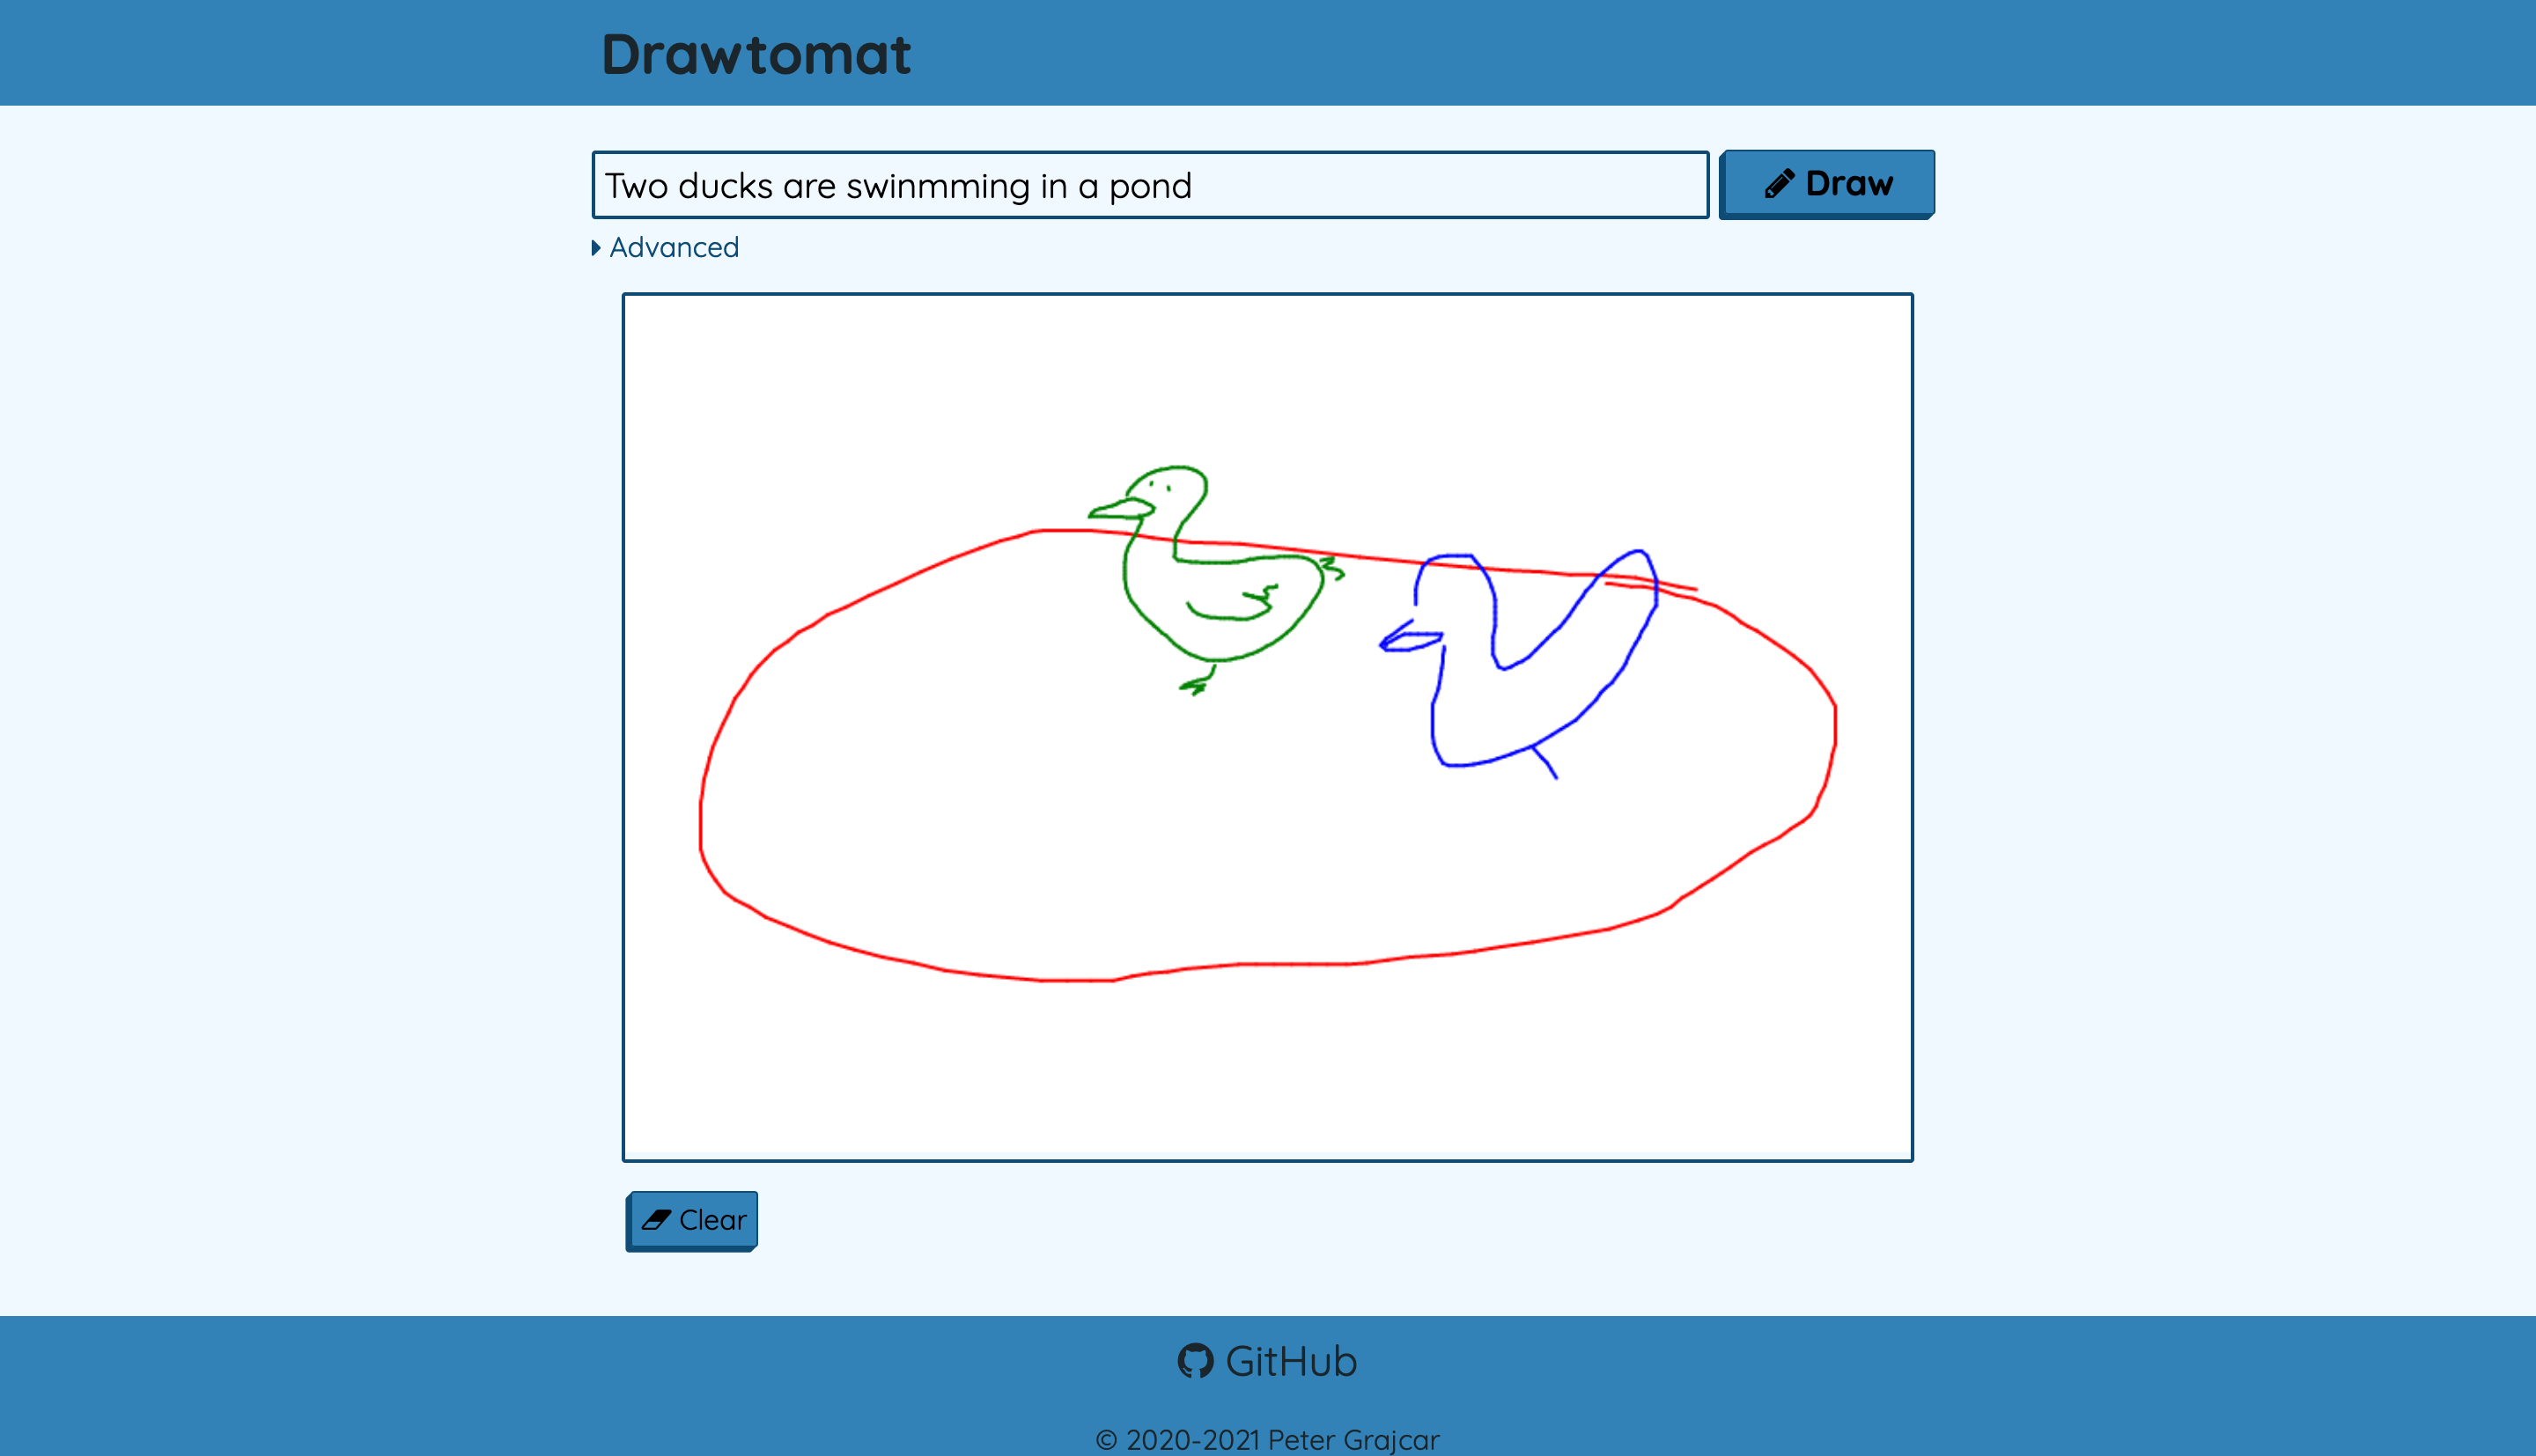
\includegraphics[width=\textwidth]{figures/web_client_1.png}
    \vskip 30pt
    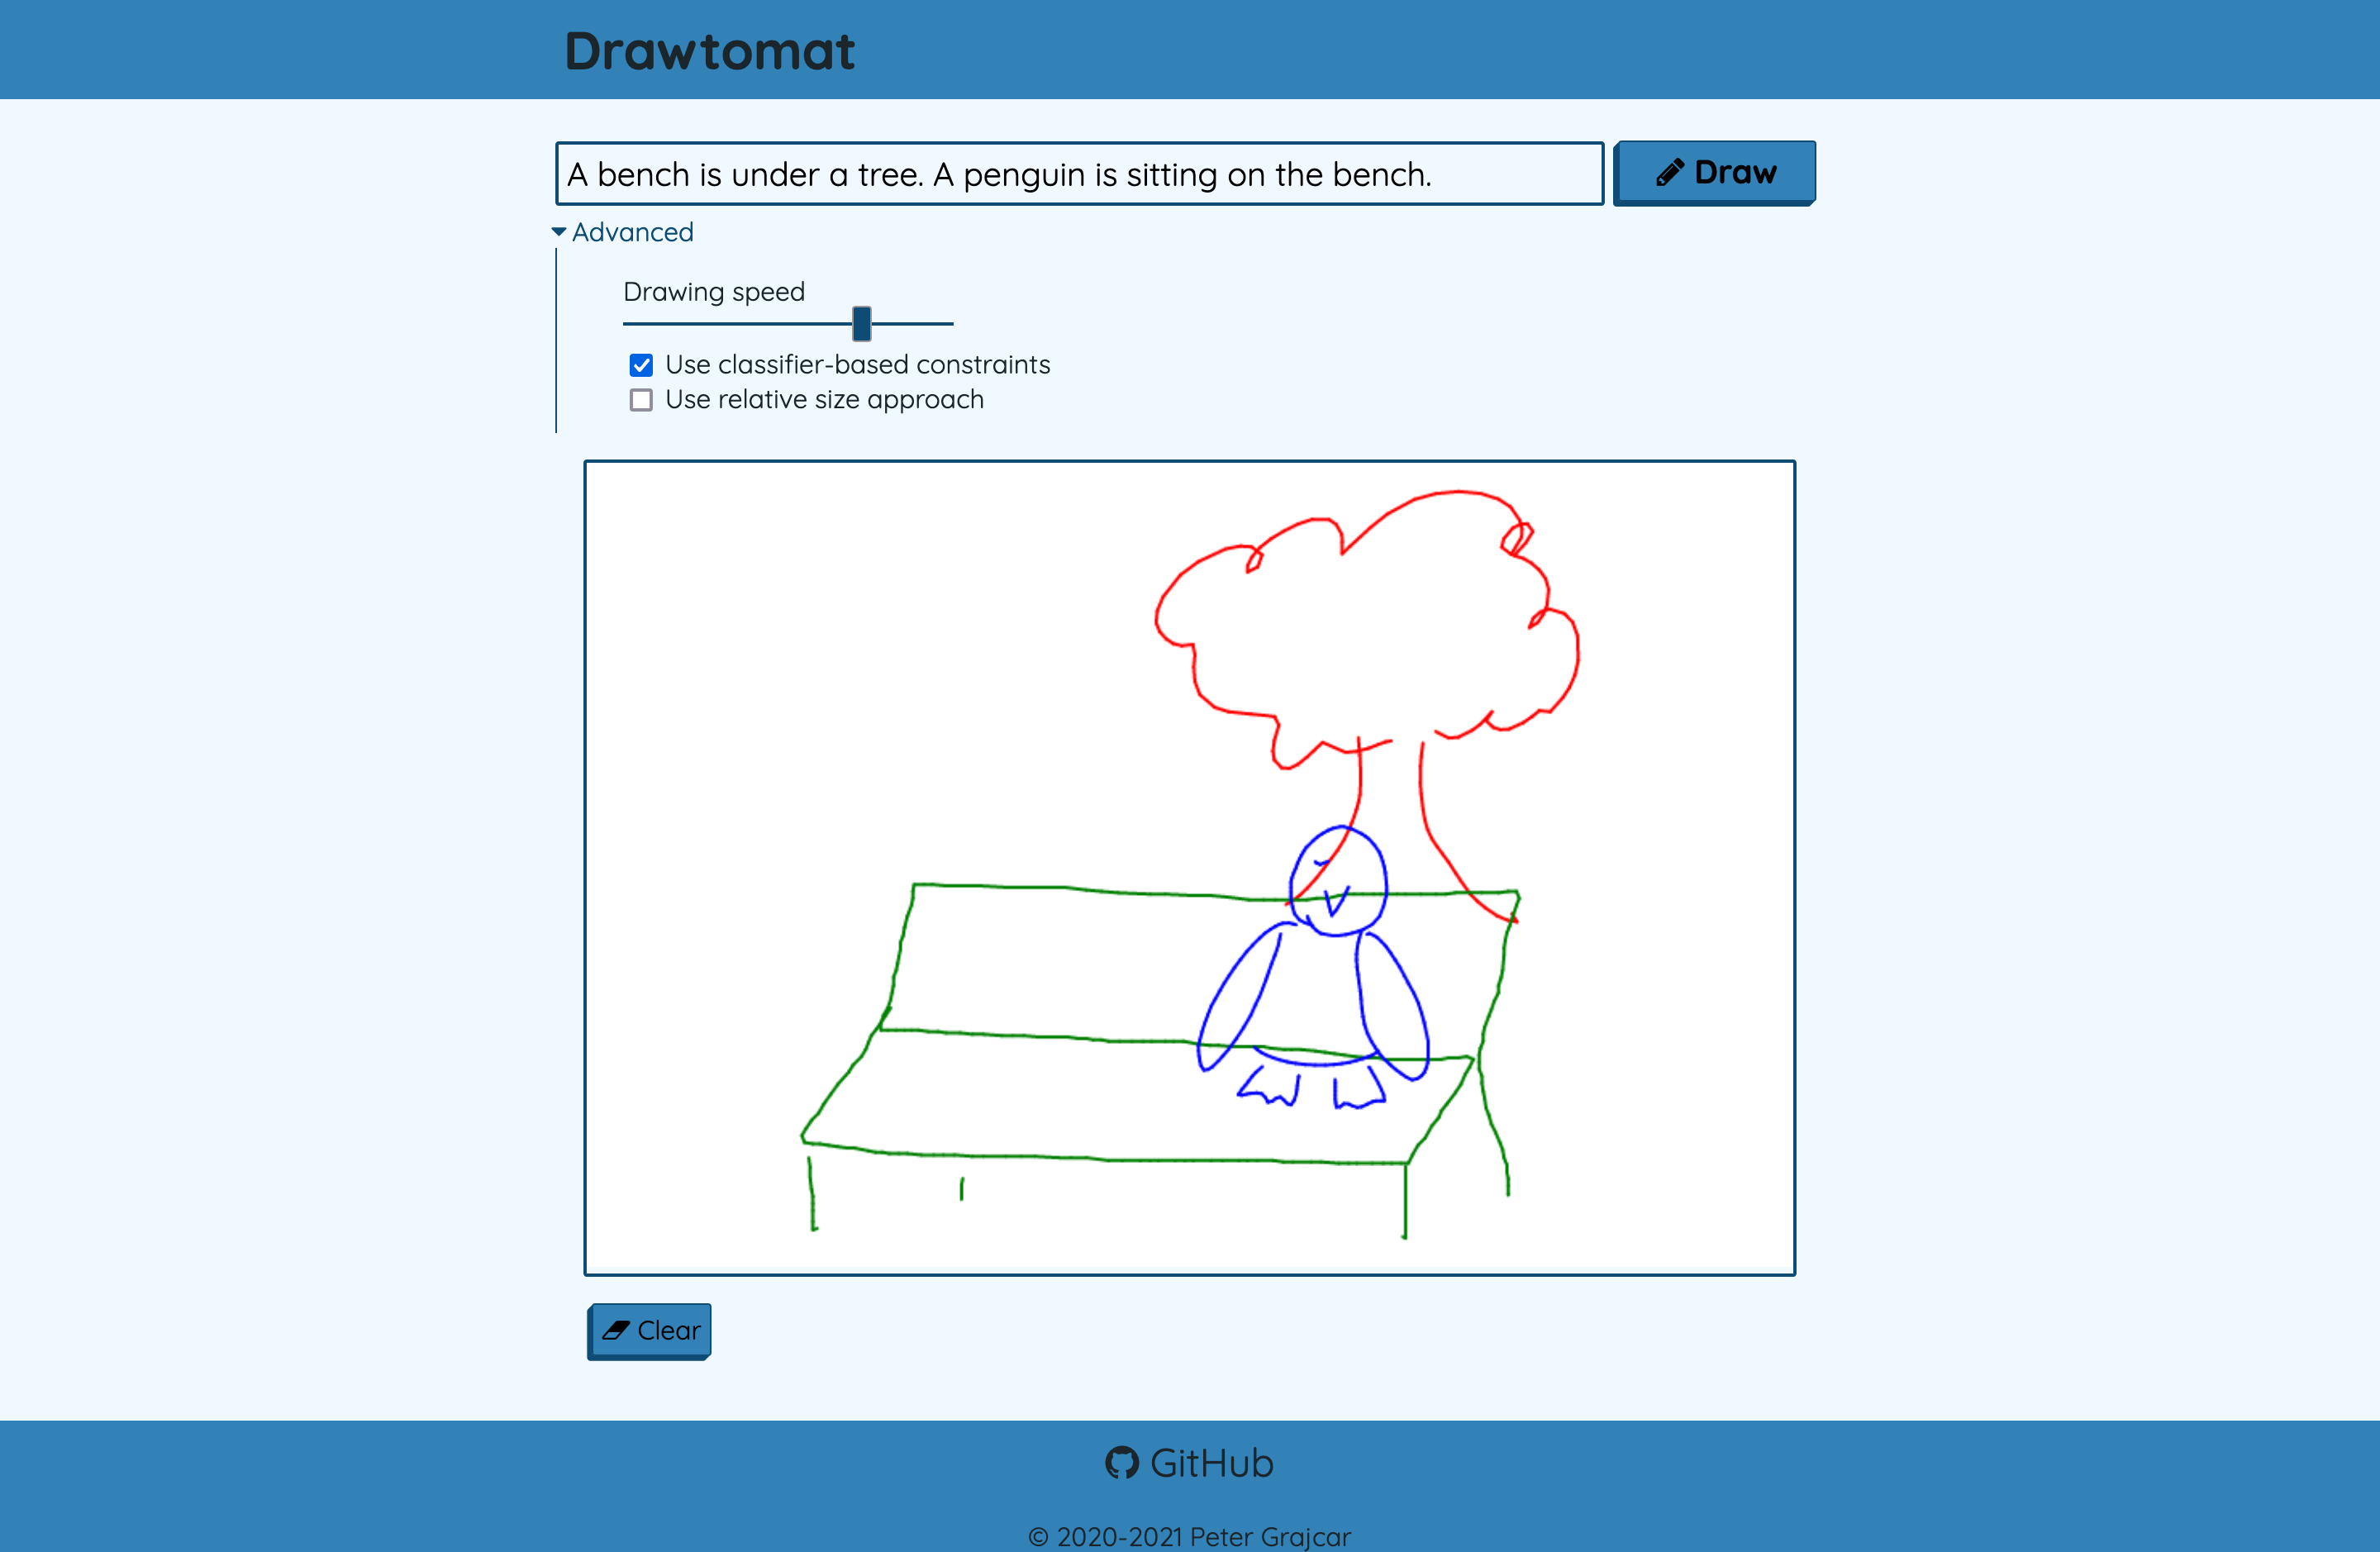
\includegraphics[width=\textwidth]{figures/web_client_2.png}
    \caption[The web client]{The web client.}
    \label{fig:web_client}
\end{figure}

\chapter{Results}

\section{Extracting Object Sizes}

In \fullref{sec:determining_obj_size}, we proposed three methods for determining object size by extracting data from the \emph{Scene Graph} \citep{xu2017scenegraph} dataset. In this section, we compare and evaluate the three methods.

\subsection{Evaluation}

The size data extracted from the \emph{Scene Graph} \citep{xu2017scenegraph} dataset using the above method are compared against the hand-written sizes. The extracted absolute sizes can be directly compared to the hand-written data. The relative sizes are compared against size ratios between the absolute hand-written sizes.

\medskip

We use the Root-Mean-Square Error (RMSE) as a metric. For $N$ predictions $y_0, \dots, y_n$ and target values $t_0, \dots, t_n$, RMSE is defined as:
\begin{align*}
    \text{RMSE} = \sqrt{\frac{1}{n}\sum_{i = 0}^n (y_i - t_i)^2}
\end{align*}

\medskip

The second metric we are interested in is the percentage of covered pairs, i.e., for how many pairs, out of the total of $119\,025$ pairs, we were able to extract the size data.

\subsection{Quantitative and Qualitative Results}

The RMSEs of the proposed size extraction methods are reported in Tables \ref{tab:sizeextraction:1} and \ref{tab:sizeextraction:2}. \Cref{tab:sizeextraction:1} compares variants of the proposed methods with transitive closures.

\begin{table}[!ht]
    \centering
    \resizebox{\textwidth}{!}{
        \begin{tabular}{c|c|c|c}
            \textbf{Method} & \textbf{Width RMSE} & \textbf{Height RMSE} & \textbf{Pairs Covered} \\
            \hline \hline
            Absolute                            & $51.93$           & $43.17$           & $\textbf{91.49\%}$    \\ 
            Relative                            & $\textbf{12.97}$  & $16.46$           & $7.50\%$              \\
            Relative + word embedding           & $43.93$           & $42.46$           & $63.60\%$             \\
            Relative + word embedding (0.85)    & $19.78$           & $24.87$           & $10.34\%$             \\
            Relative + word embedding (0.95)    & $13.13$           & $\textbf{16.12}$  & $7.92\%$              \\
        \end{tabular}
    }
    \caption[Comparison of the size extraction methods]{Comparison of the size extraction methods.}
    \label{tab:sizeextraction:1}
\end{table}

\begin{table}[!ht]
    \centering
    \resizebox{\textwidth}{!}{
        \begin{threeparttable}
            \begin{tabular}{c|c|c|c}
                \textbf{Method} & \textbf{Width RMSE} & \textbf{Height RMSE} & \textbf{Pairs Covered} \\
                \hline \hline
                Absolute$^*$                        & $51.93$           & $43.17$           & $91.49\%$         \\ 
                Relative                            & $\textbf{43.65}$  & $\textbf{41.04}$  & $79.70\%$         \\
                Relative + word embedding           & $55.53$           & $47.92$           & $\textbf{100\%}$  \\
                Relative + word embedding (0.85)    & $53.35$           & $45.65$           & $86.57\%$         \\
                Relative + word embedding (0.95)    & $49.39$           & $42.03$           & $82.30\%$         \\
            \end{tabular}
            \begin{tablenotes}
            \small
            \item $^*$ Transitive closure cannot be applied to the absolute sizes. The results are the same as in \Cref{tab:sizeextraction:2}. For the sake of comparison, they are also included in this table.
            \end{tablenotes}
        \end{threeparttable}
    }
    \caption[Comparison of the size extraction methods with transitive closure]{Comparison of the size extraction methods with transitive closure.}
    \label{tab:sizeextraction:2}
\end{table}

All relative size methods outperformed the absolute size method in terms of RMSE. However, these methods cover significantly fewer pairs. The transitive closure partially solves the small pair coverage problem, but it also introduces larger errors. Similarly, the word embeddings helped to increase both the pair coverage and errors.

\begin{figure}[ht]
    \centering
        \begin{subfigure}{0.45\textwidth}
            \centering
            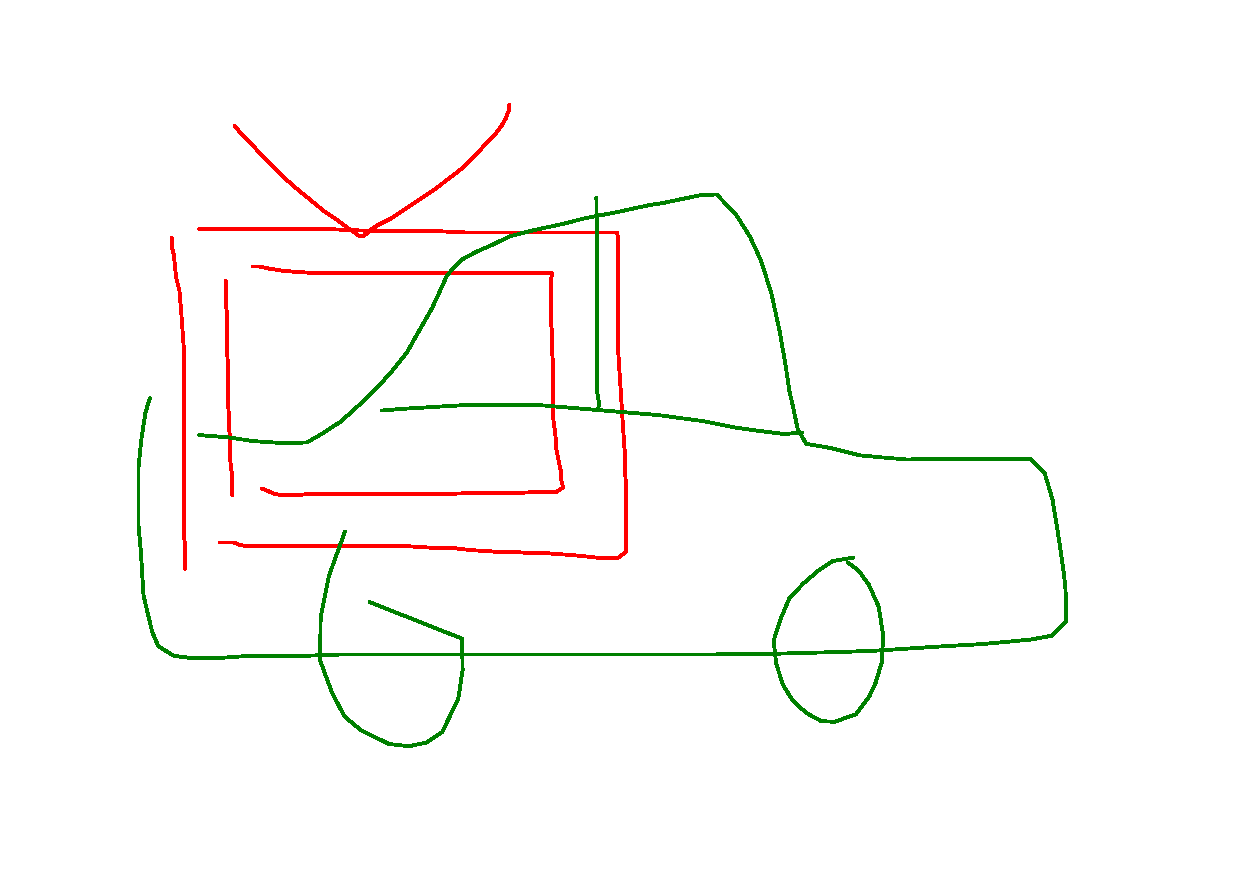
\includegraphics[width=\textwidth]{figures/car_on_tv_abs.pdf}
        \end{subfigure}
        \begin{subfigure}{0.45\textwidth}
            \centering
            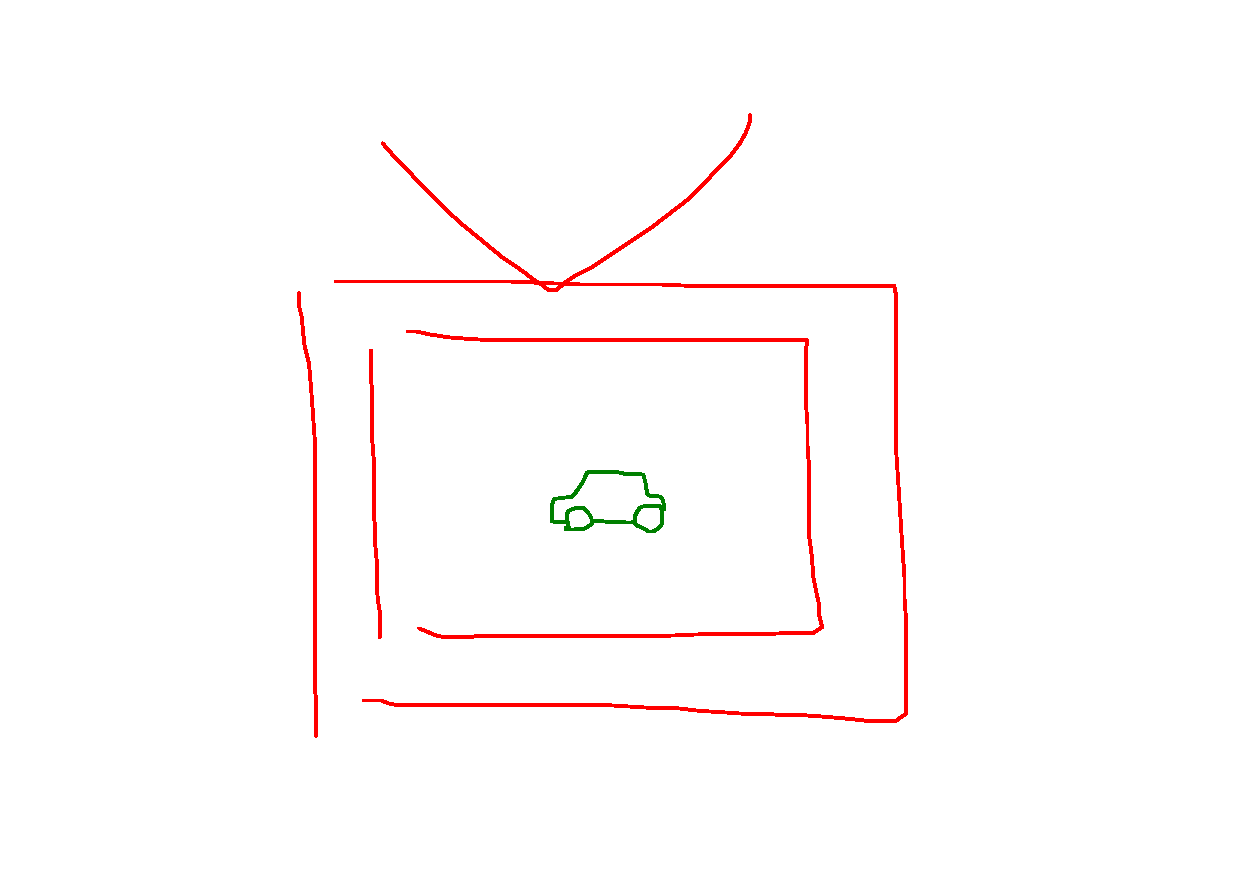
\includegraphics[width=\textwidth]{figures/car_on_tv_rel.pdf}
        \end{subfigure}
    \caption[Comparison of absolute and relative size method]{Drawings generated from description \protect\say{A car is on the television.} using absolute (right) and relative (left) sizes.}
    \label{fig:absolute_vs_relative}
\end{figure}

\begin{figure}[ht]
    \centering
    \captionsetup[subfigure]{labelformat=empty}
        \begin{subfigure}{0.45\textwidth}
            \centering
            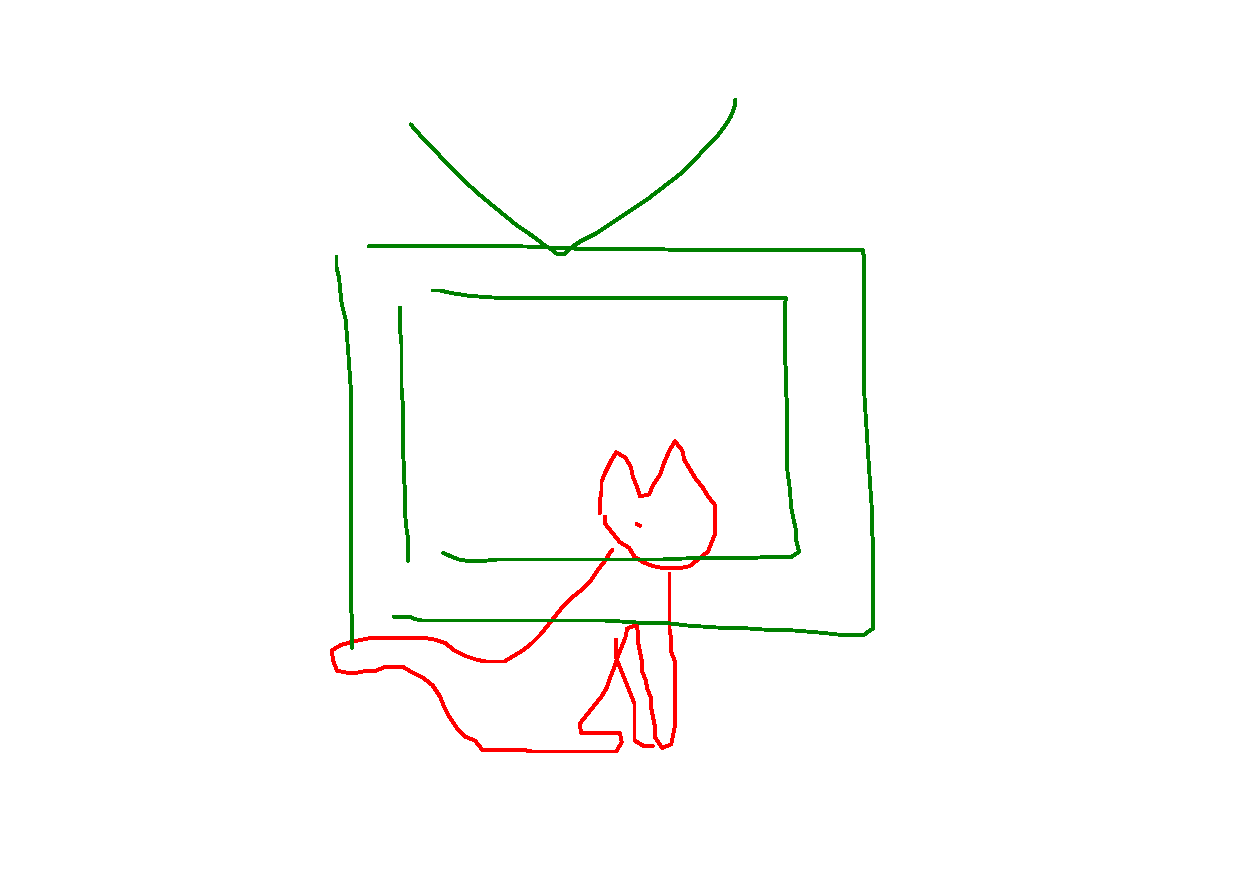
\includegraphics[width=\textwidth]{figures/television_behind_cat.pdf}
            \caption{\protect\say{A television is behind a cat.}}
        \end{subfigure}
        \hfill
        \begin{subfigure}{0.45\textwidth}
            \centering
            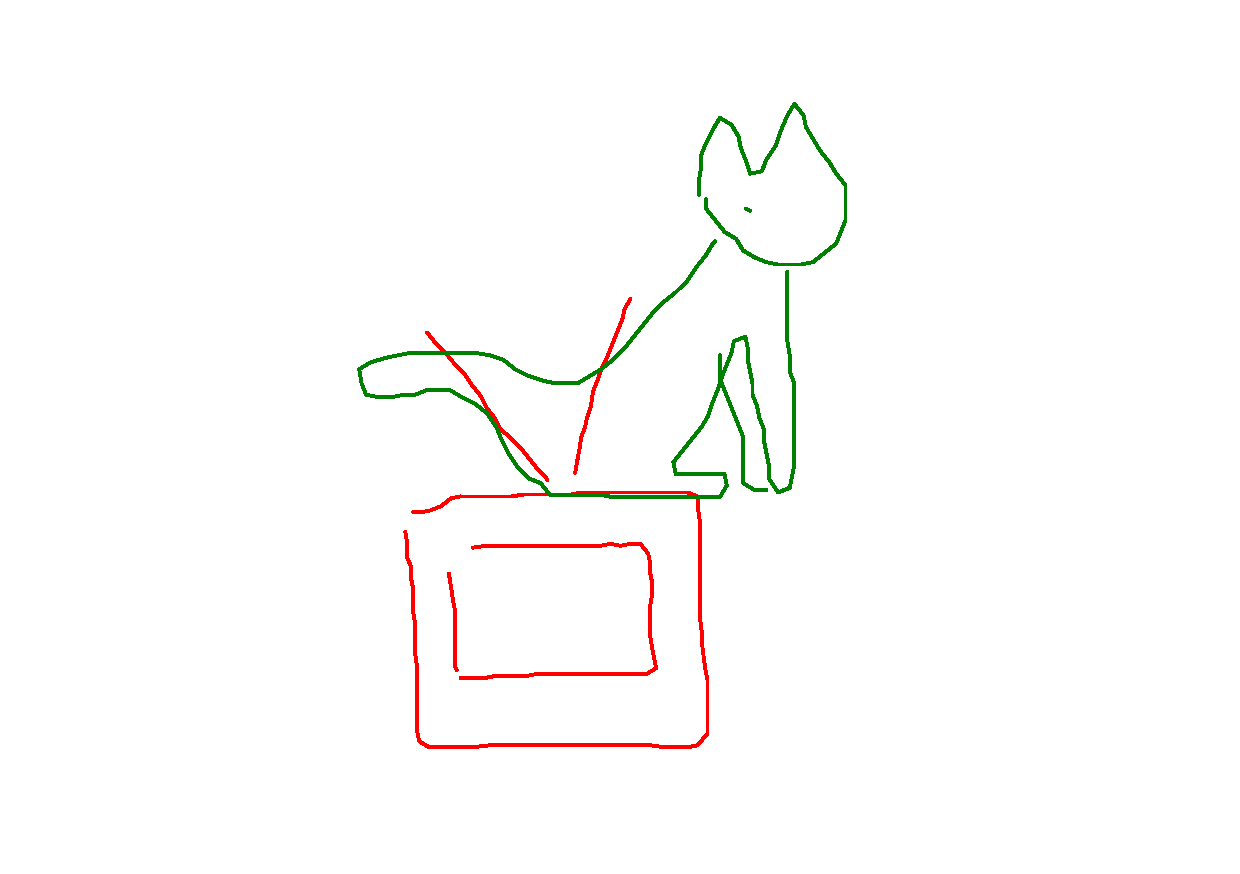
\includegraphics[width=\textwidth]{figures/cat_on_television.pdf}
            \caption{\protect\say{A cat is sitting on a television.}}
        \end{subfigure}
        
        \begin{subfigure}{0.45\textwidth}
            \centering
            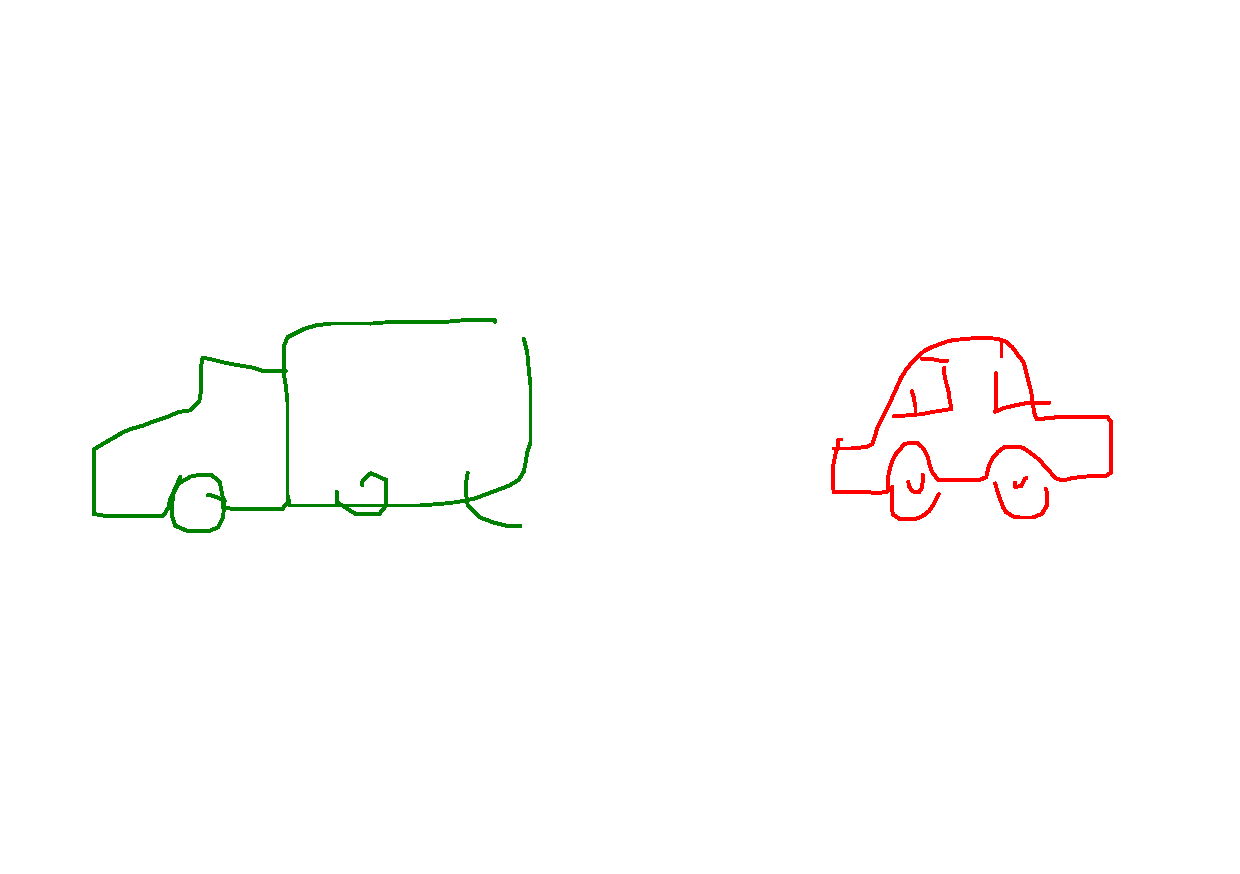
\includegraphics[width=\textwidth]{figures/truck_behind_car.pdf}
            \caption{\protect\say{A truck is behind a car.}}
        \end{subfigure}
        \hfill
        \begin{subfigure}{0.45\textwidth}
            \centering
            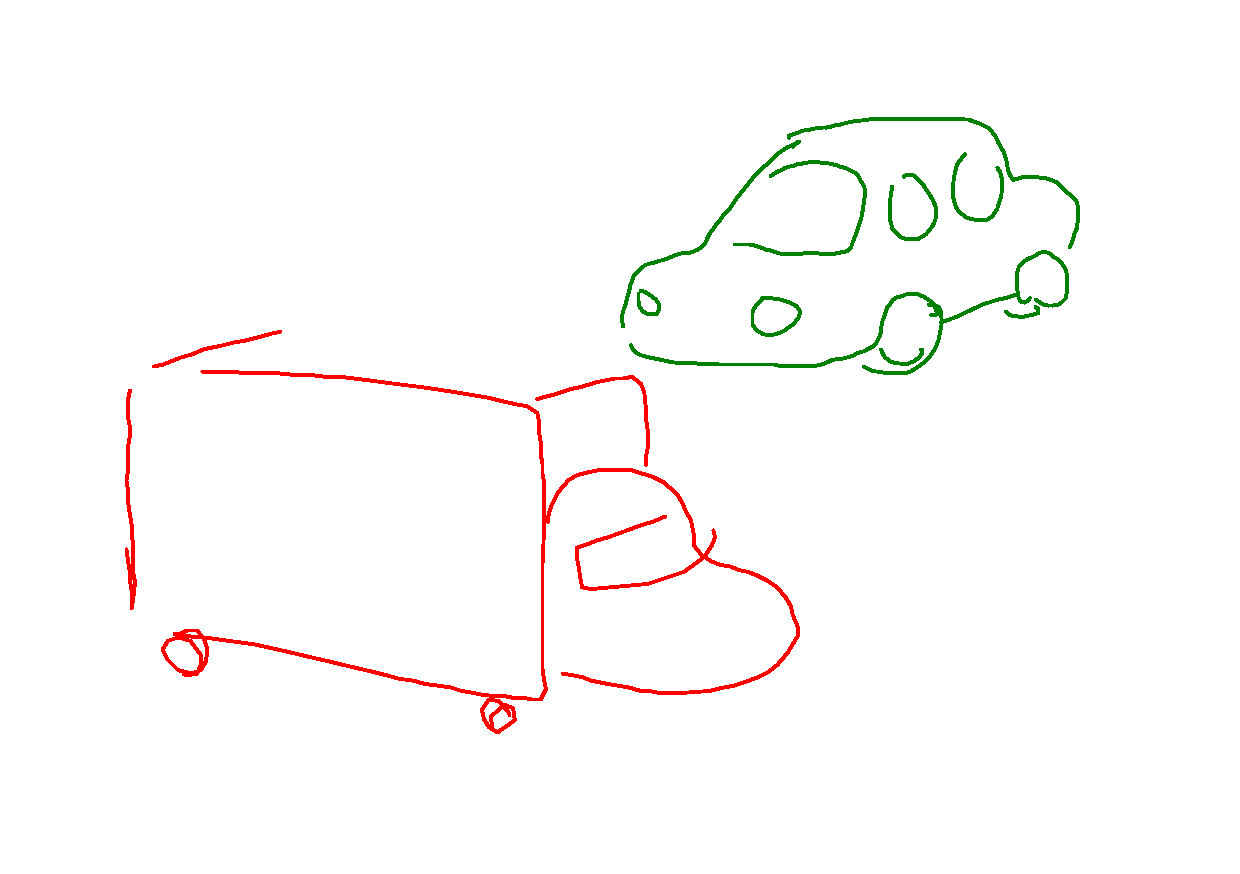
\includegraphics[width=\textwidth]{figures/car_next_to_truck.pdf}
            \caption{\protect\say{A car is next to a truck.}}
        \end{subfigure}
       
        \begin{subfigure}{0.45\textwidth}
            \centering
            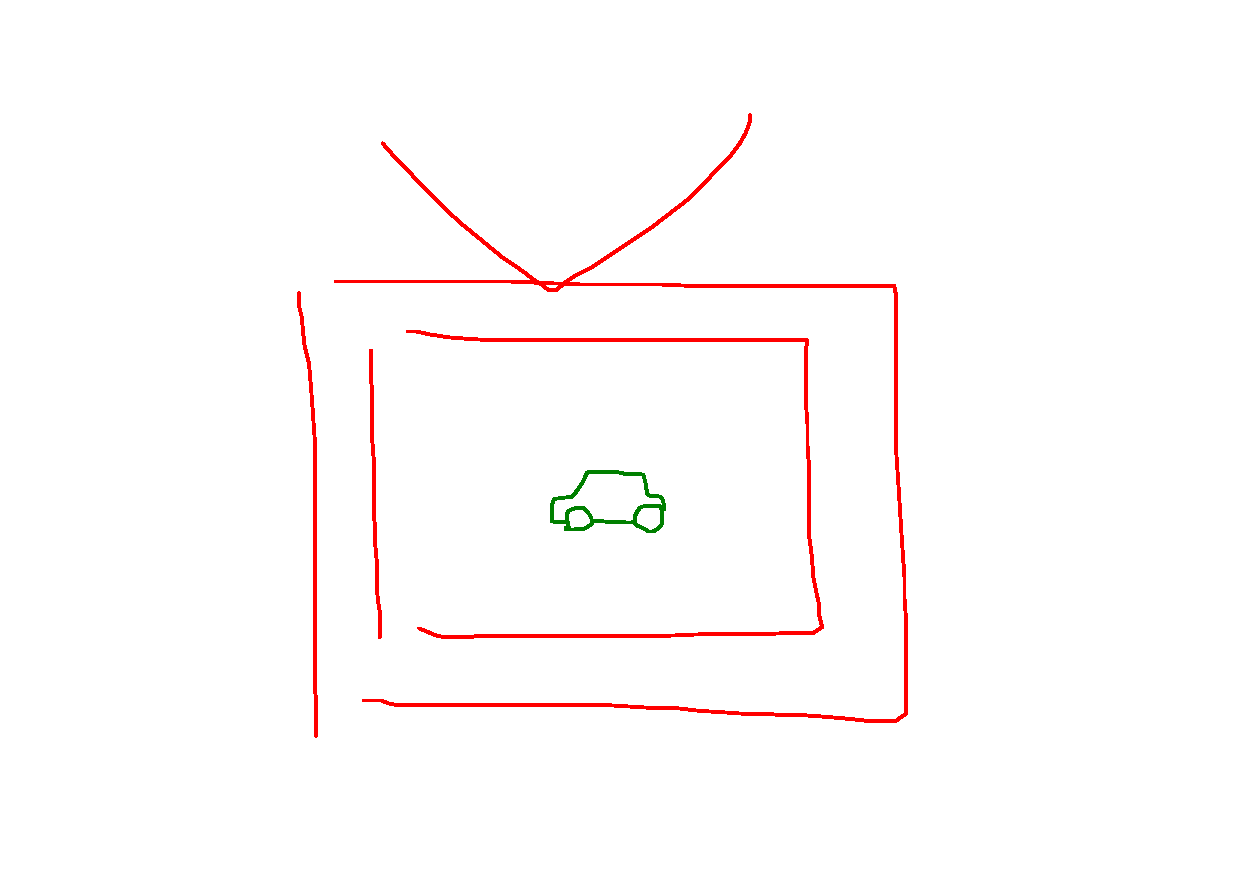
\includegraphics[width=\textwidth]{figures/car_on_tv_rel.pdf}
            \caption{\protect\say{A car is on the television.}}
        \end{subfigure}
        \hfill
        \begin{subfigure}{0.45\textwidth}
            \centering
            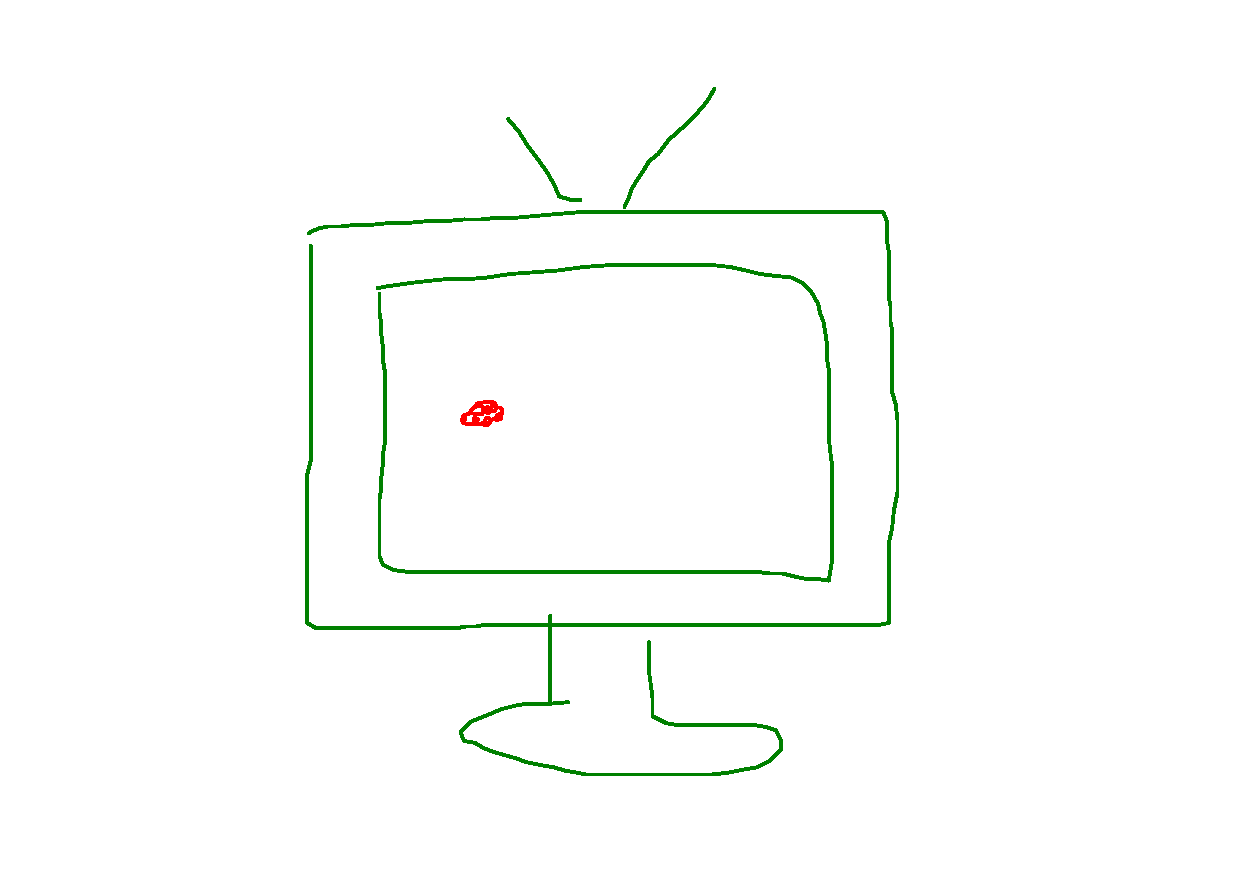
\includegraphics[width=\textwidth]{figures/television_in_front_of_car.pdf}
            \caption{\protect\say{A television is in front of a car.}}
        \end{subfigure}
    \caption[Drawings generated using the relative size method]{Drawings generated using the relative size method.}
    \label{fig:relative_size_examples}
\end{figure}

\Cref{fig:absolute_vs_relative} compares the absolute size and relative size methods on the example given in \Cref{sec:determining_obj_size}. In this particular example, the relative size method addresses the problem stated in the mentioned section. However, the rightmost drawing in \Cref{fig:relative_size_examples} shows that the method fails the other way around. Presumably, the dataset captures certain pairs of objects only in a narrow variety of contexts, leading to biased estimations. Furthermore, the relative size approach is oblivious to the predicates associated with the relation. We have chosen not to include the predicate as it would vastly decrease the pair coverage.

\section{Positional Constraints}
\label{sec:constraint_results}

In \Cref{sec:rule_based_constraints} and \Cref{sec:classifier_based_constraints}, we introduced a rule-based and a classifier-based approach for determining the objects' positions. In this section, we compare those two approaches.

\medskip

The first version of the classifier-based approach considers only the predicate and the relative position described in \Cref{sec:classifier_based_constraints}. As shown in \Cref{fig:boundaries:3}, constraints implemented using this classifier closely resemble the rule-based alternatives. It shows that the \emph{Scene Graph} \citep{xu2017scenegraph} dataset is a viable source of semantic information about the connection of predicates and mutual positions of objects. The figure also suggests that this classifier is a sufficient replacement for the simple rule-based approach.

\medskip

The second version of the classifier takes into account the semantic subject. \Cref{fig:boundaries:2} shows that this classifier can capture different semantics of a predicate with respect to the subject. More examples are shown in \Cref{fig:boundaries:5}. 

\medskip

The major drawback of the classifier-based approach is the lack of information about the shape of the object. This problem is partially illustrated by \Cref{fig:boundaries:4}. In some cases, the rule-based approach provides more precise boundaries than the classifier-based alternative.

\begin{figure}[ht]
    \centering
        \begin{subfigure}{0.45\textwidth}
            \centering
            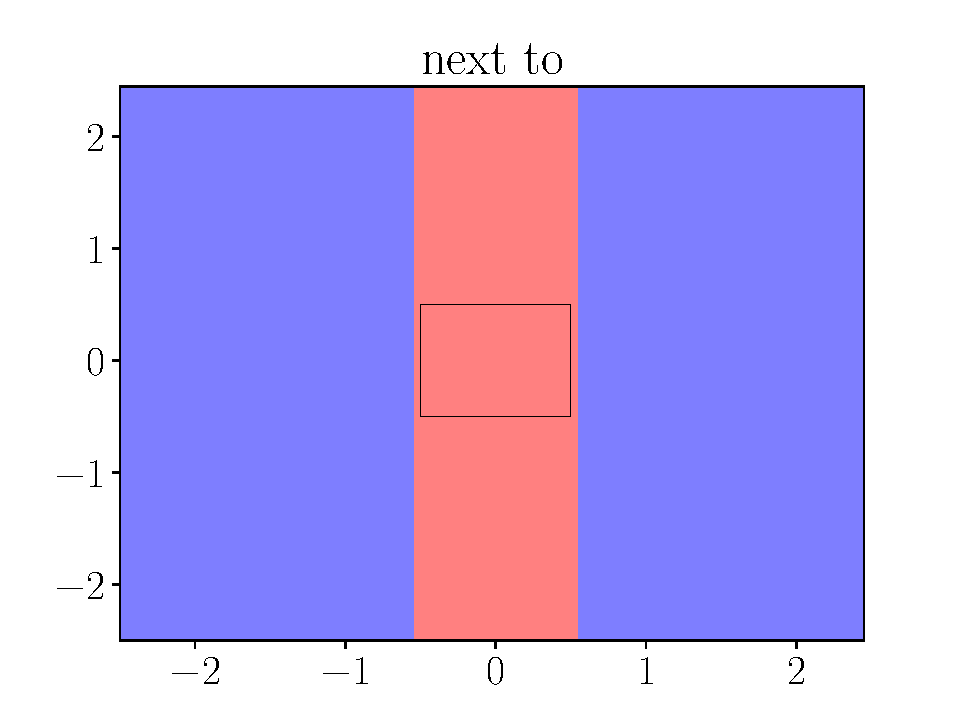
\includegraphics[width=\textwidth]{figures/next_to_rule.pdf}
        \end{subfigure}
        \begin{subfigure}{0.45\textwidth}
            \centering
            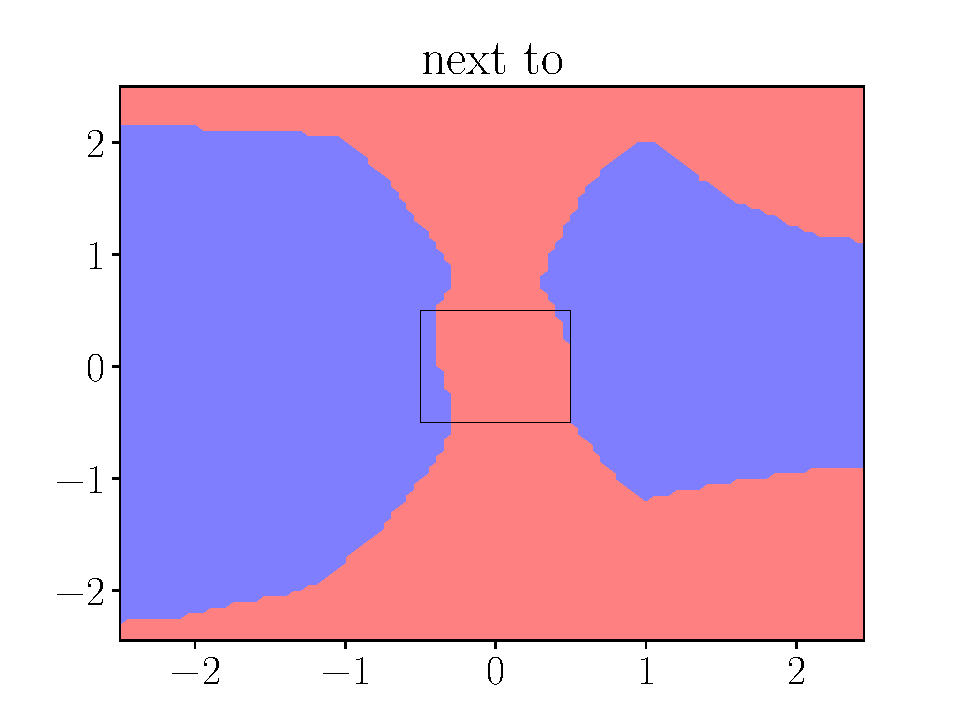
\includegraphics[width=\textwidth]{figures/next_to_predicate_only.pdf}
        \end{subfigure}
        \begin{subfigure}{0.45\textwidth}
            \centering
            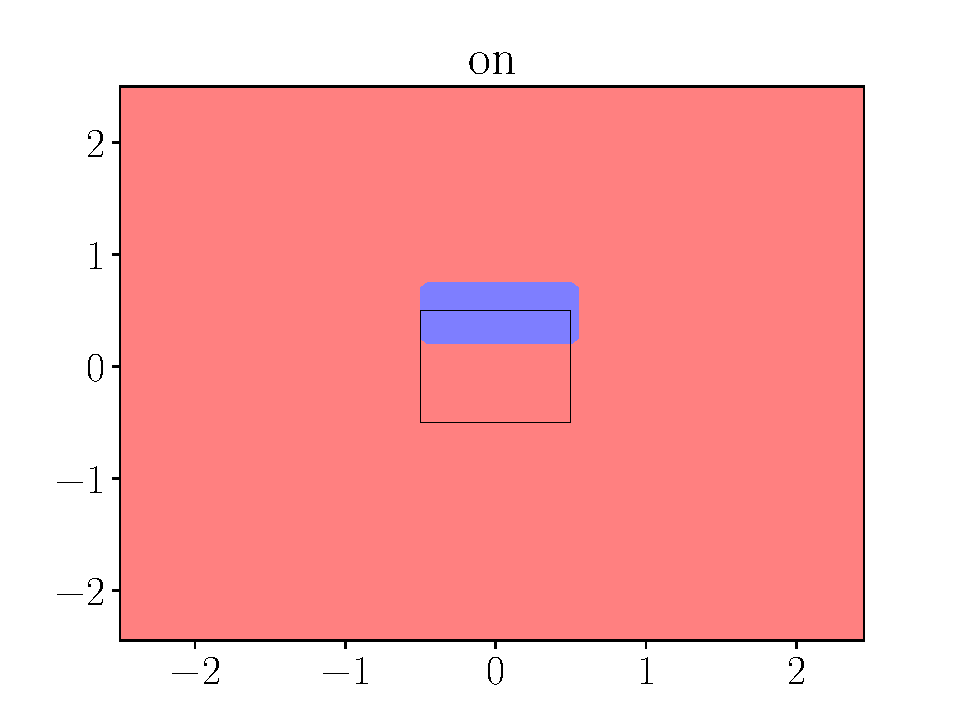
\includegraphics[width=\textwidth]{figures/on_rule.pdf}
        \end{subfigure}
        \begin{subfigure}{0.45\textwidth}
            \centering
            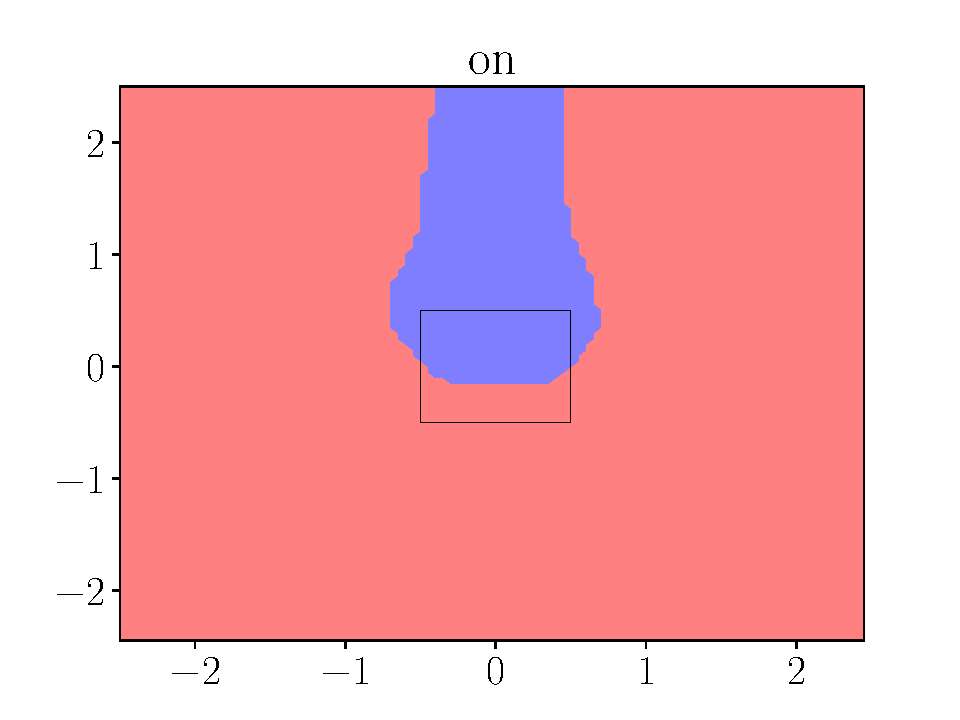
\includegraphics[width=\textwidth]{figures/on_predicate_only.pdf}
        \end{subfigure}
        \begin{subfigure}{0.45\textwidth}
            \centering
            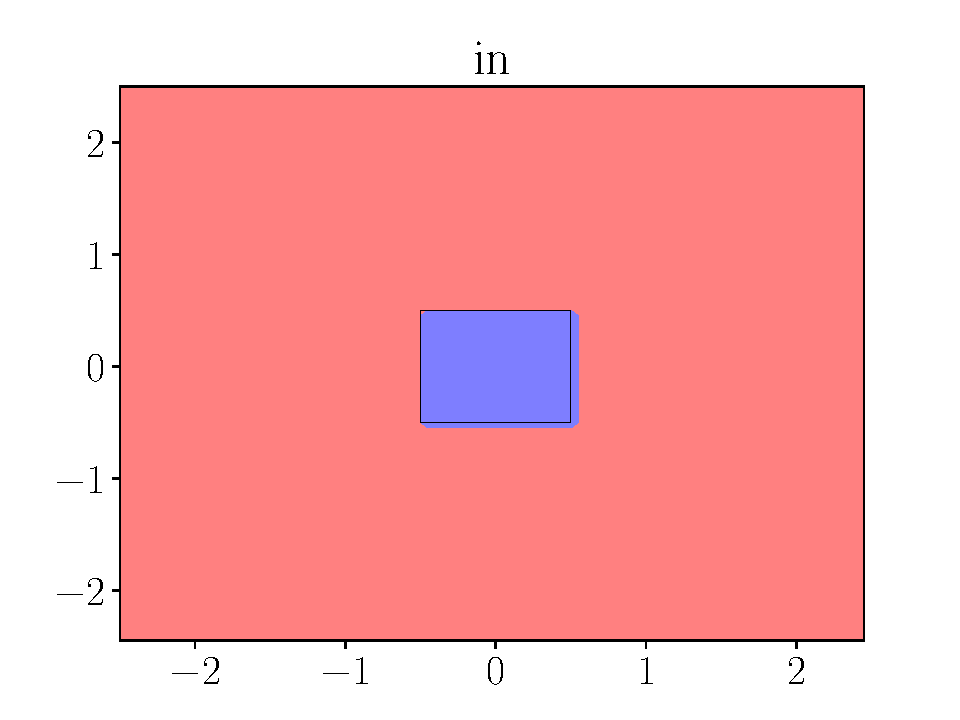
\includegraphics[width=\textwidth]{figures/in_rule.pdf}
        \end{subfigure}
        \begin{subfigure}{0.45\textwidth}
            \centering
            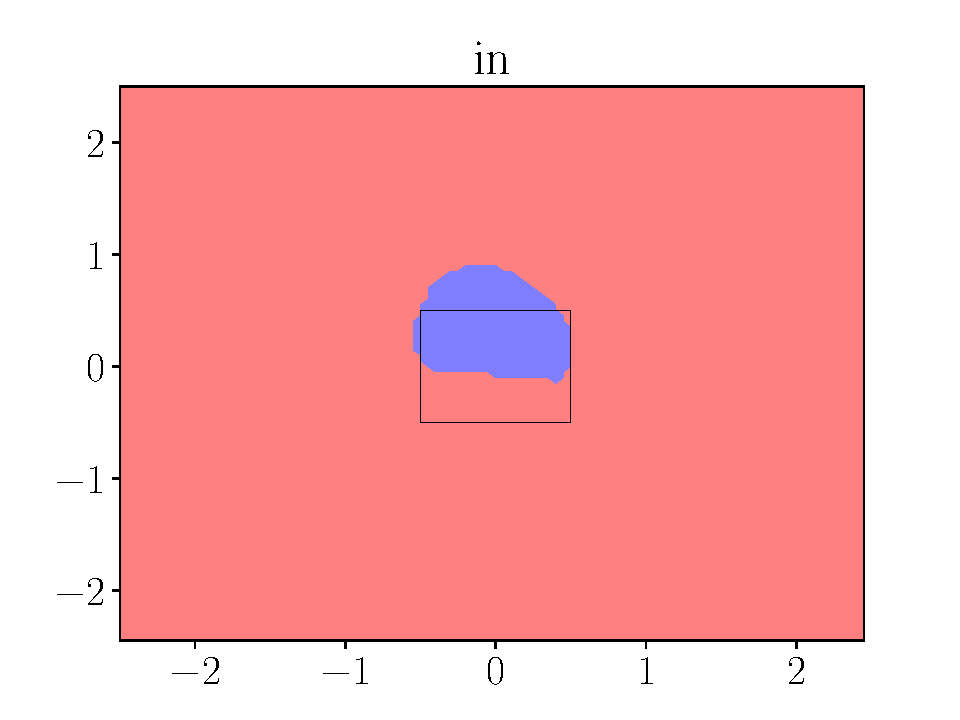
\includegraphics[width=\textwidth]{figures/in_predicate_only.pdf}
        \end{subfigure}
        \begin{subfigure}{0.45\textwidth}
            \centering
            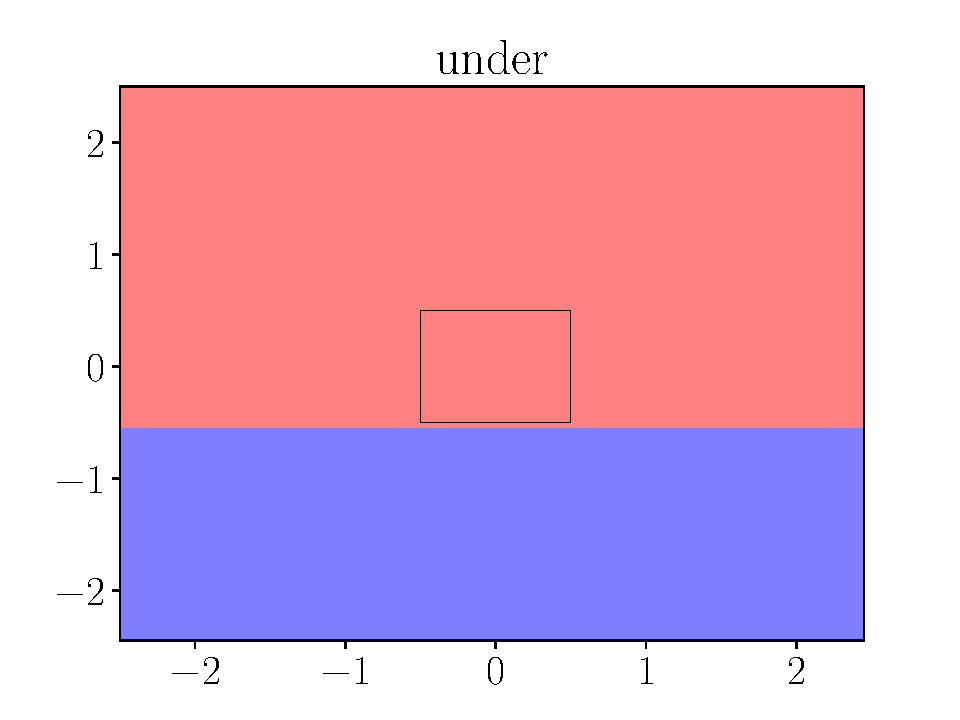
\includegraphics[width=\textwidth]{figures/under_rule.pdf}
        \end{subfigure}
        \begin{subfigure}{0.45\textwidth}
            \centering
            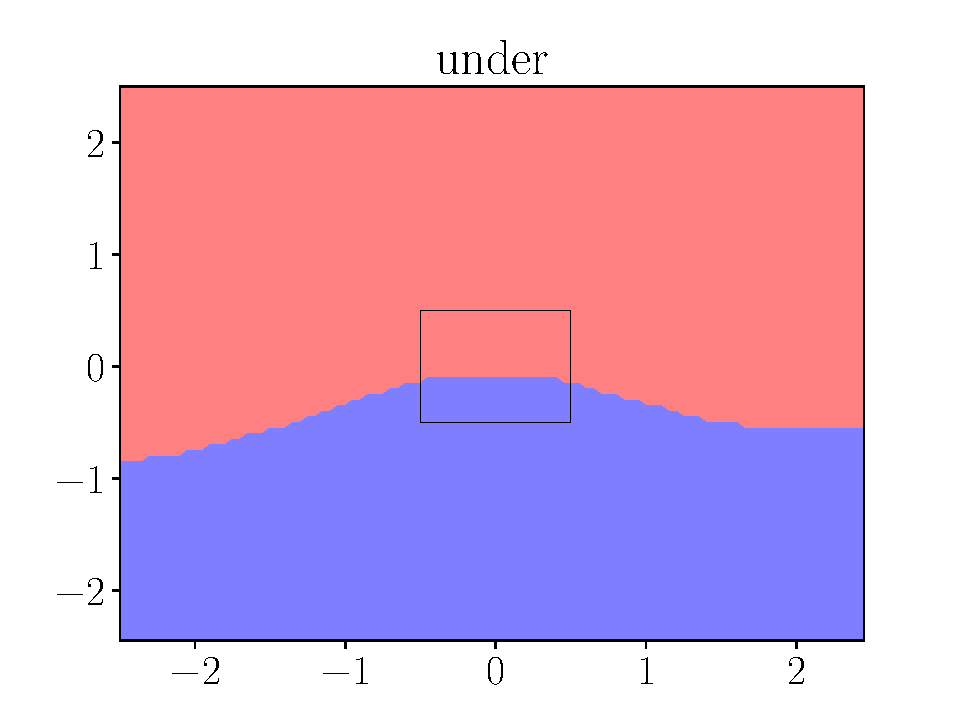
\includegraphics[width=\textwidth]{figures/under_predicate_only.pdf}
        \end{subfigure}
    \caption[Rule-based constraints compared to classifier-based constraints]{Rule-based constraints (on the left) compared to the classifier-based constraints (on the right). The classifier used in these examples was trained using only predicates and the $x$, $y$ coordinates.}
    \label{fig:boundaries:3}
\end{figure}

\begin{figure}[ht]
    \centering
        \begin{subfigure}{0.45\textwidth}
            \centering
            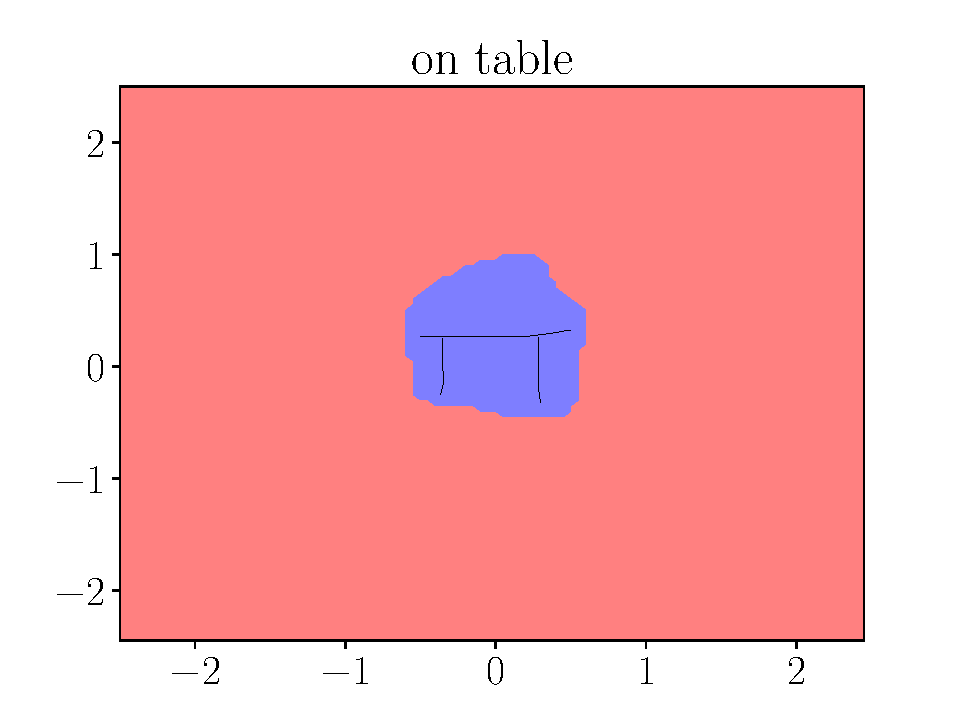
\includegraphics[width=\textwidth]{figures/on_table}
        \end{subfigure}
        \begin{subfigure}{0.45\textwidth}
            \centering
            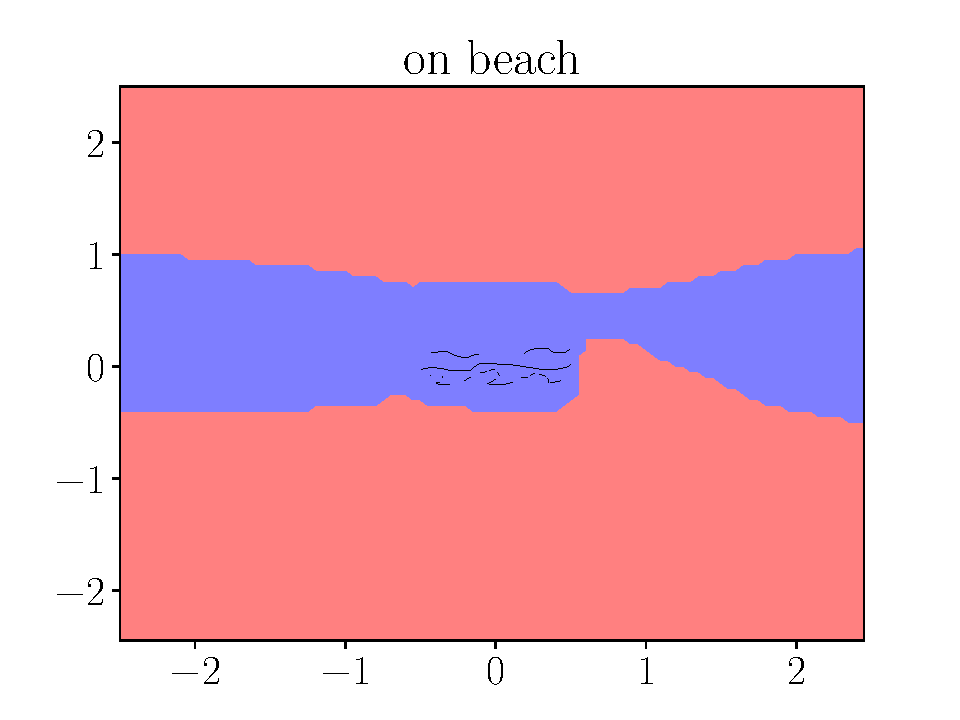
\includegraphics[width=\textwidth]{figures/on_beach}
        \end{subfigure}
    \caption[Different decision boundaries for the same predicate]{Different decision boundaries capture semantic difference of the same predicate in different contexts.}
    \label{fig:boundaries:2}
\end{figure}

\begin{figure}[ht]
    \centering
        \begin{subfigure}{0.45\textwidth}
            \centering
            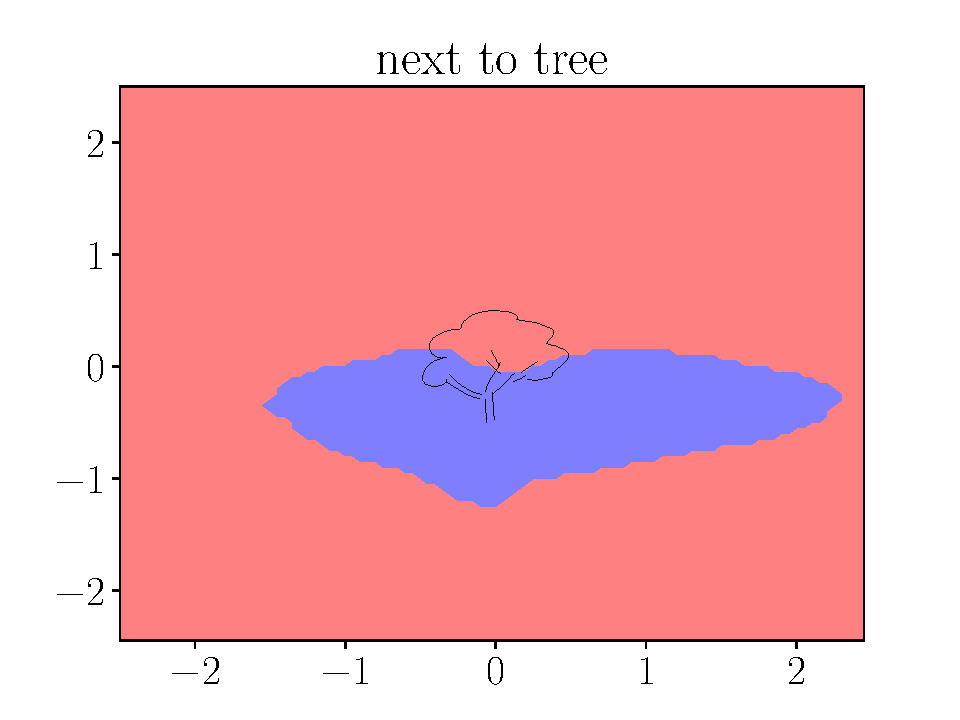
\includegraphics[width=\textwidth]{figures/next_to_tree.pdf}
        \end{subfigure}
        \begin{subfigure}{0.45\textwidth}
            \centering
            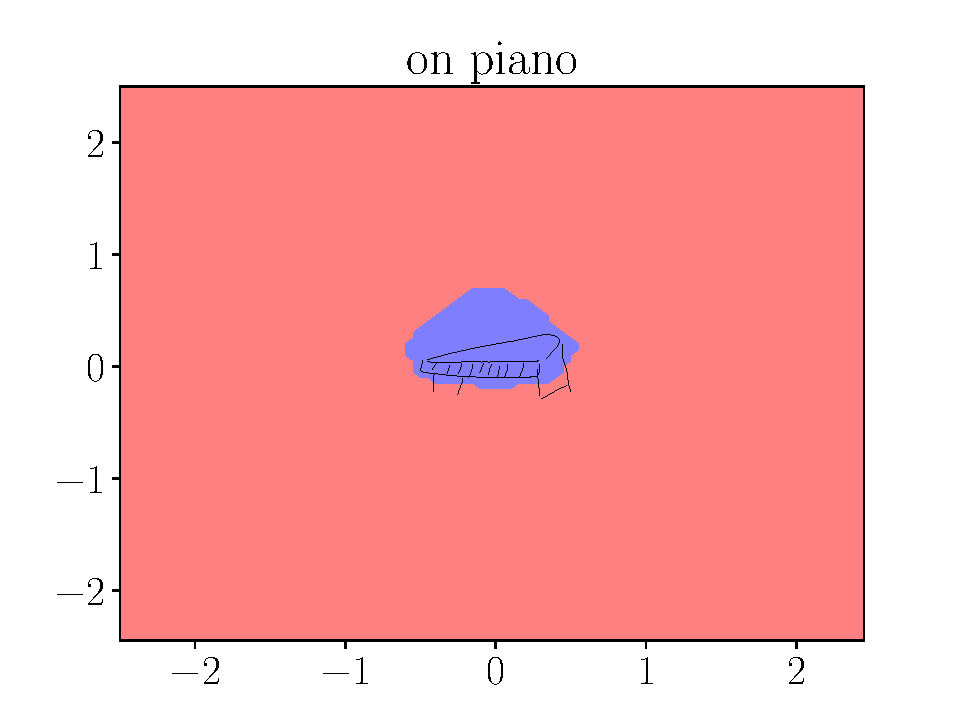
\includegraphics[width=\textwidth]{figures/on_piano.pdf}
        \end{subfigure}
        \begin{subfigure}{0.45\textwidth}
            \centering
            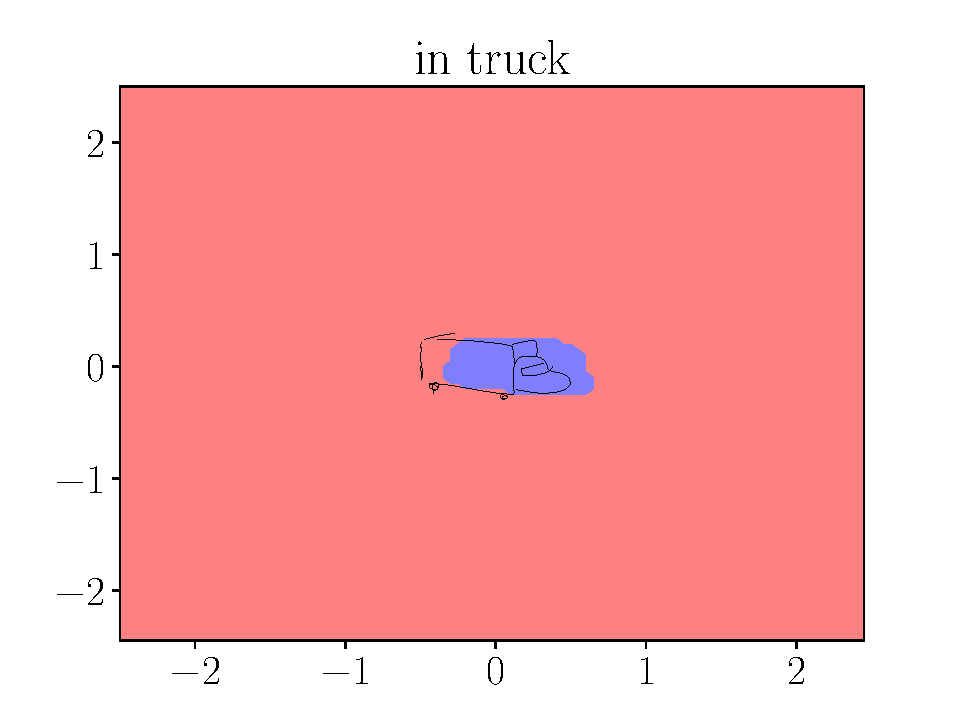
\includegraphics[width=\textwidth]{figures/in_truck.pdf}
        \end{subfigure}
        \begin{subfigure}{0.45\textwidth}
            \centering
            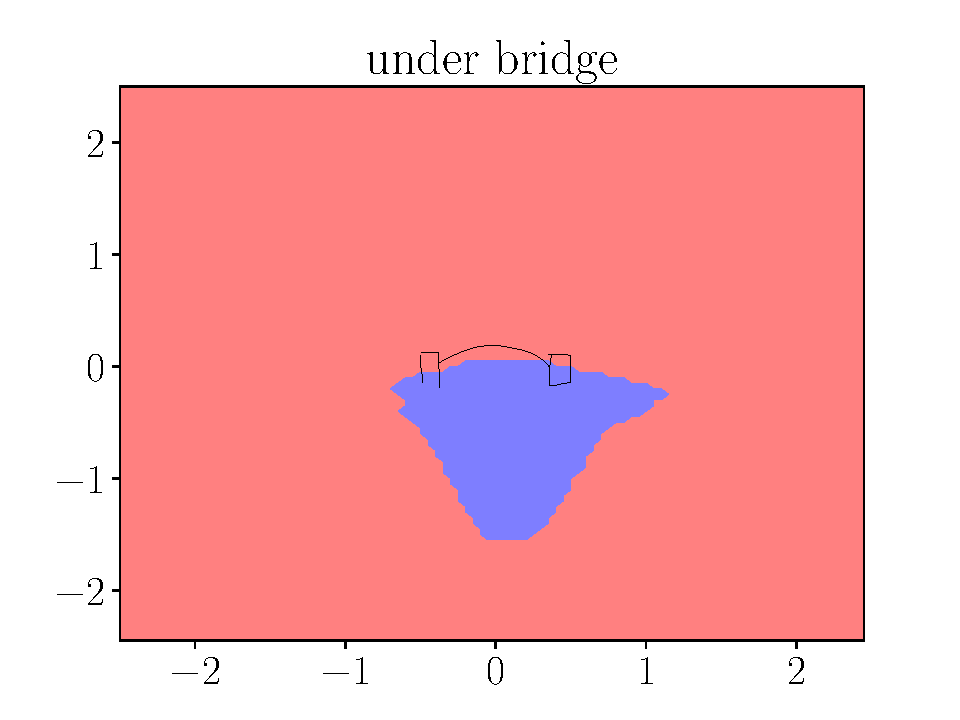
\includegraphics[width=\textwidth]{figures/under_bridge.pdf}
        \end{subfigure}
    \caption[More examples of the classifier-based constraints]{More examples of the classifier-based constraints.}
    \label{fig:boundaries:5}
\end{figure}

\begin{figure}[ht]
    \centering
        \begin{subfigure}{0.45\textwidth}
            \centering
            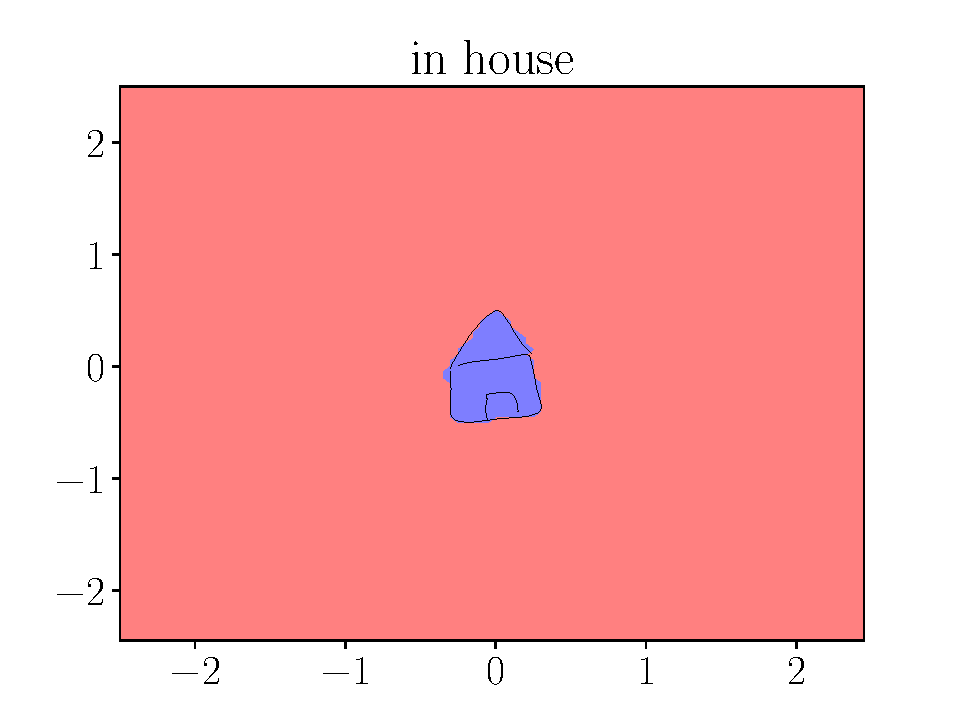
\includegraphics[width=\textwidth]{figures/in_house_rule.pdf}
        \end{subfigure}
        \begin{subfigure}{0.45\textwidth}
            \centering
            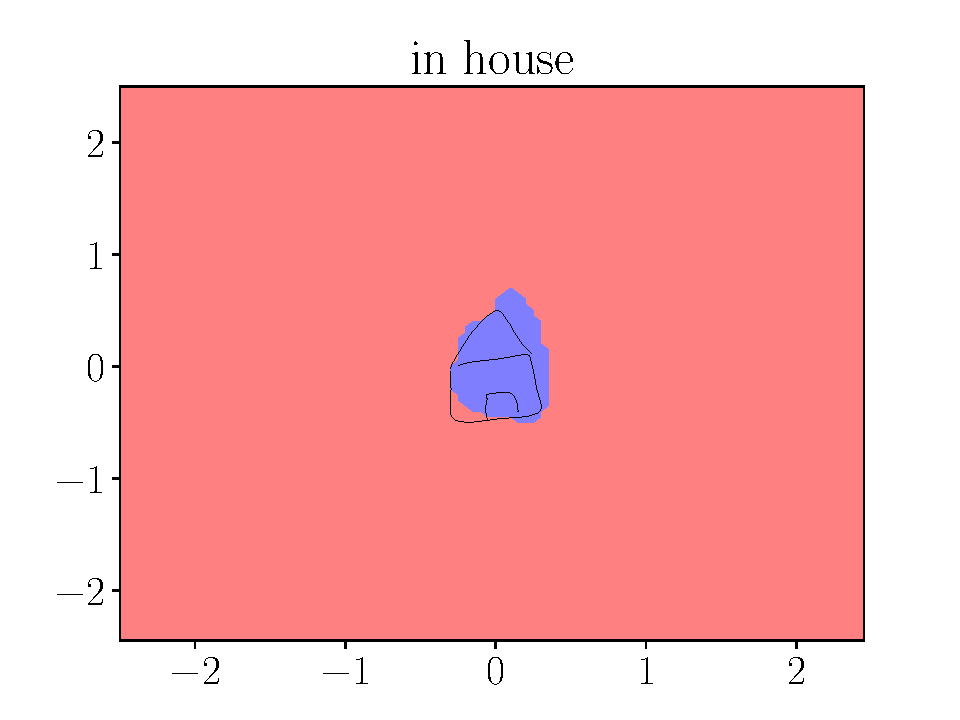
\includegraphics[width=\textwidth]{figures/in_house_classifier.pdf}
        \end{subfigure}
    \caption[\emph{Inside} constraint comparison]{The rule-based \emph{inside} constraint (on the left) can be more precise than the classifier-based one (on the right).}
    \label{fig:boundaries:4}
\end{figure}


\chapter{Discussion}

None of the approaches compared in the preceding chapter is flawless, and each works better under certain circumstances. Our implementation gives the user an option to choose the approach and experiment with the results. \Cref{fig:composed_drawings} shows that in many cases, the results are similar across different selected approaches. The random nature of the Monte Carlo algorithm allows generating multiple different drawings for one description. This randomness increases the chances that the generated image will eventually correspond with the input description. Future research might focus on automatic scoring and cherry-picking of the generated scenes. Other possible improvements may be achieved by employing more advanced machine-learning models used for constraints and size prediction. Our implementation relies on a simple rule-based description processing which is sufficient for simple sentences; However, finding a better approach may also be a subject of future research.

\begin{figure}[ht]
    \captionsetup[subfigure]{labelformat=empty}
    \centering
        \begin{subfigure}{\textwidth}
            \centering
            \caption{(1) \say{A dog and a cat are sitting on a couch. The couch is in a house and there is a tree next to the house.}}
            \begin{subfigure}[t]{0.45\textwidth}
                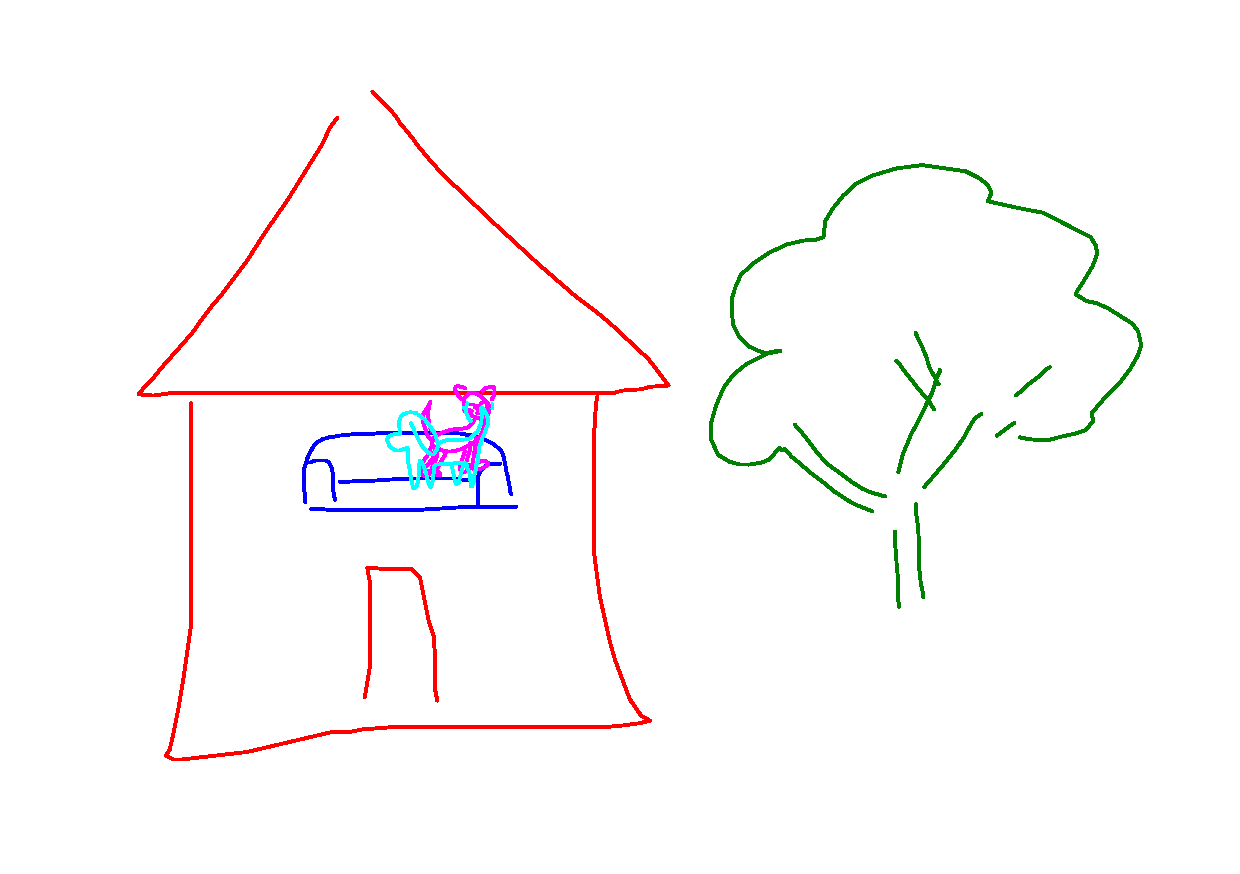
\includegraphics[width=\textwidth]{figures/drawing_1_ra.pdf}
                \caption{rule-based constraints, absolute sizes}
            \end{subfigure}
            \hfill
            \begin{subfigure}[t]{0.45\textwidth}
                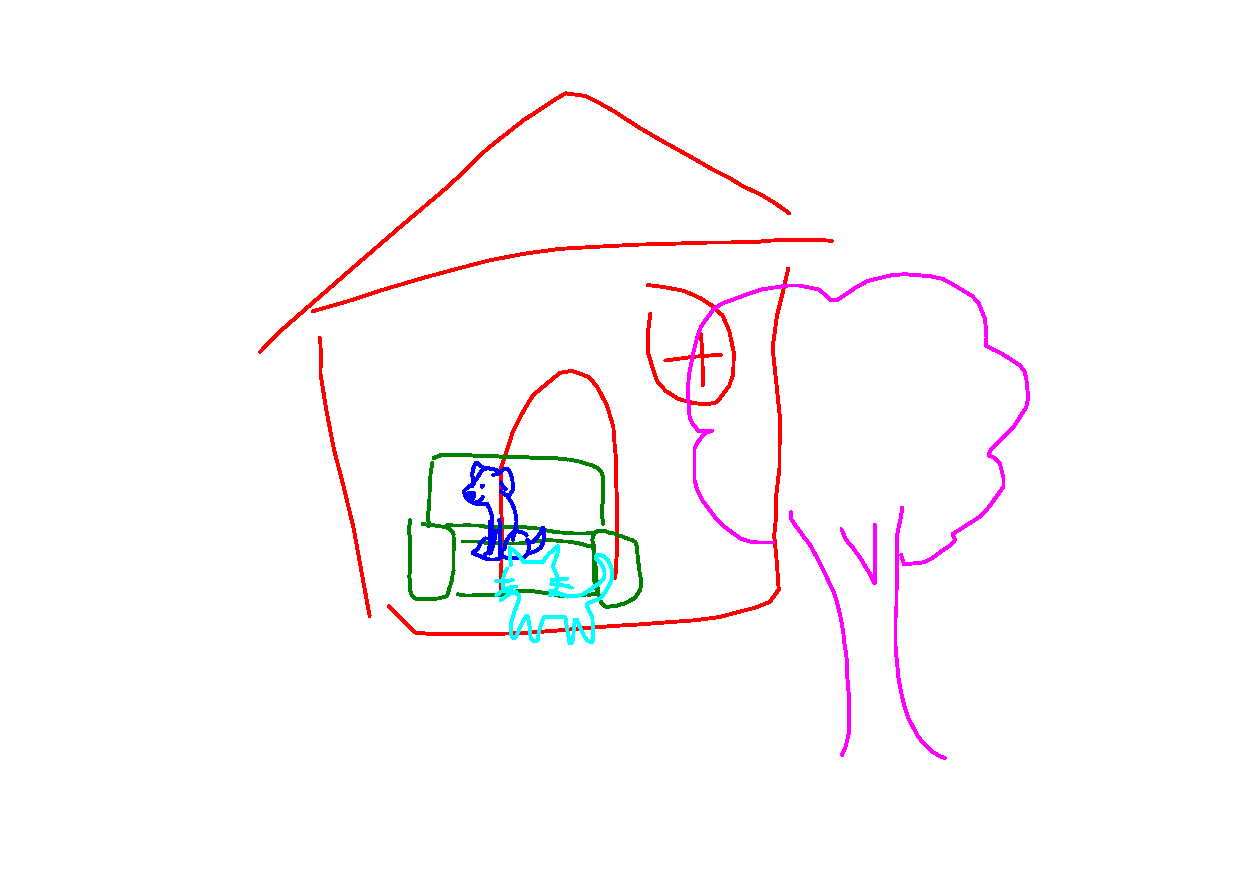
\includegraphics[width=\textwidth]{figures/drawing_1_ca.pdf}
                \caption{classifier-based constraints, absolute sizes}
            \end{subfigure}
        \end{subfigure}
        \begin{subfigure}{\textwidth}
            \centering
            \caption{(2) \say{Two ducks are swimming in a pond which is next to a tree. a bench is under the tree.}}
            \begin{subfigure}{0.45\textwidth}
                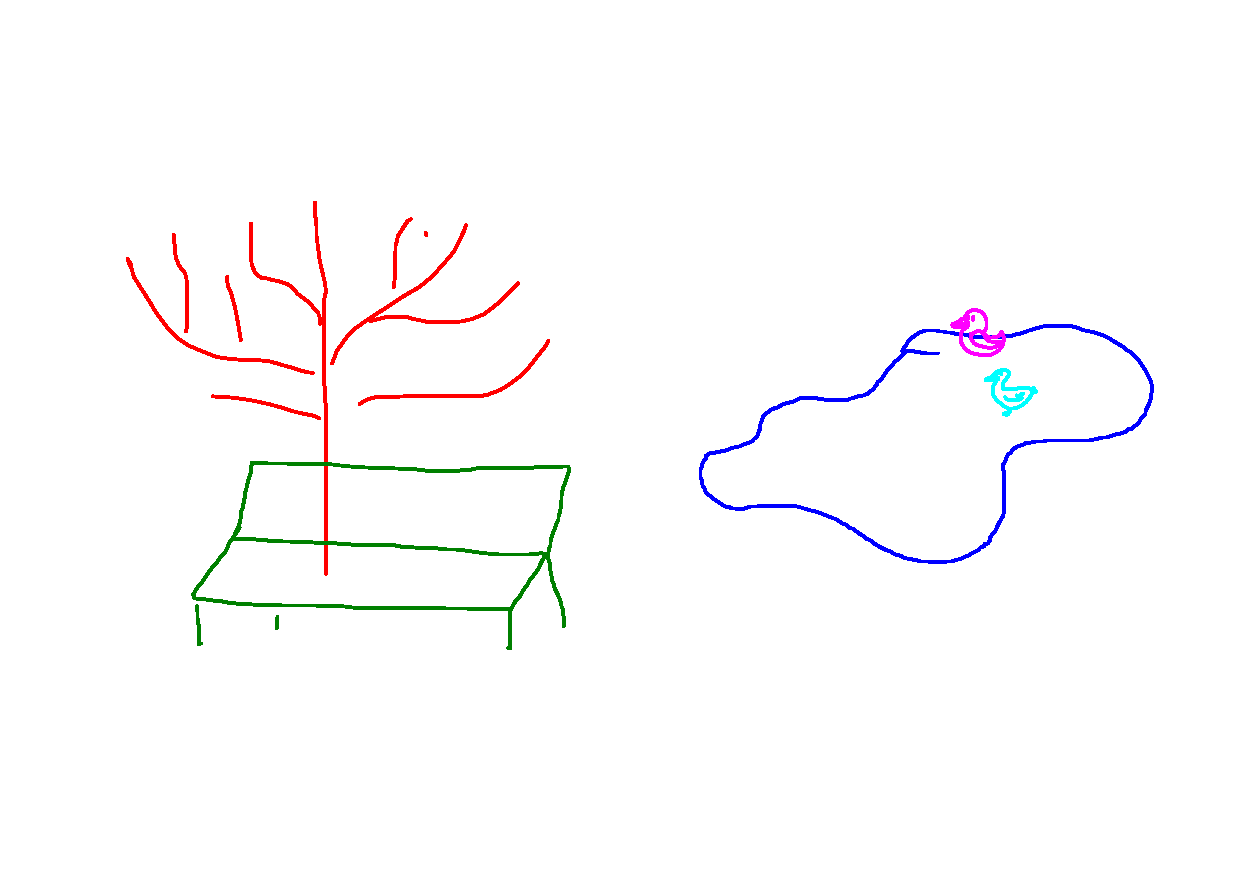
\includegraphics[width=\textwidth]{figures/drawing_2_ca.pdf}
                \caption{classifier-based constraints, absolute sizes}
            \end{subfigure} 
            \hfill
            \begin{subfigure}{0.45\textwidth}
                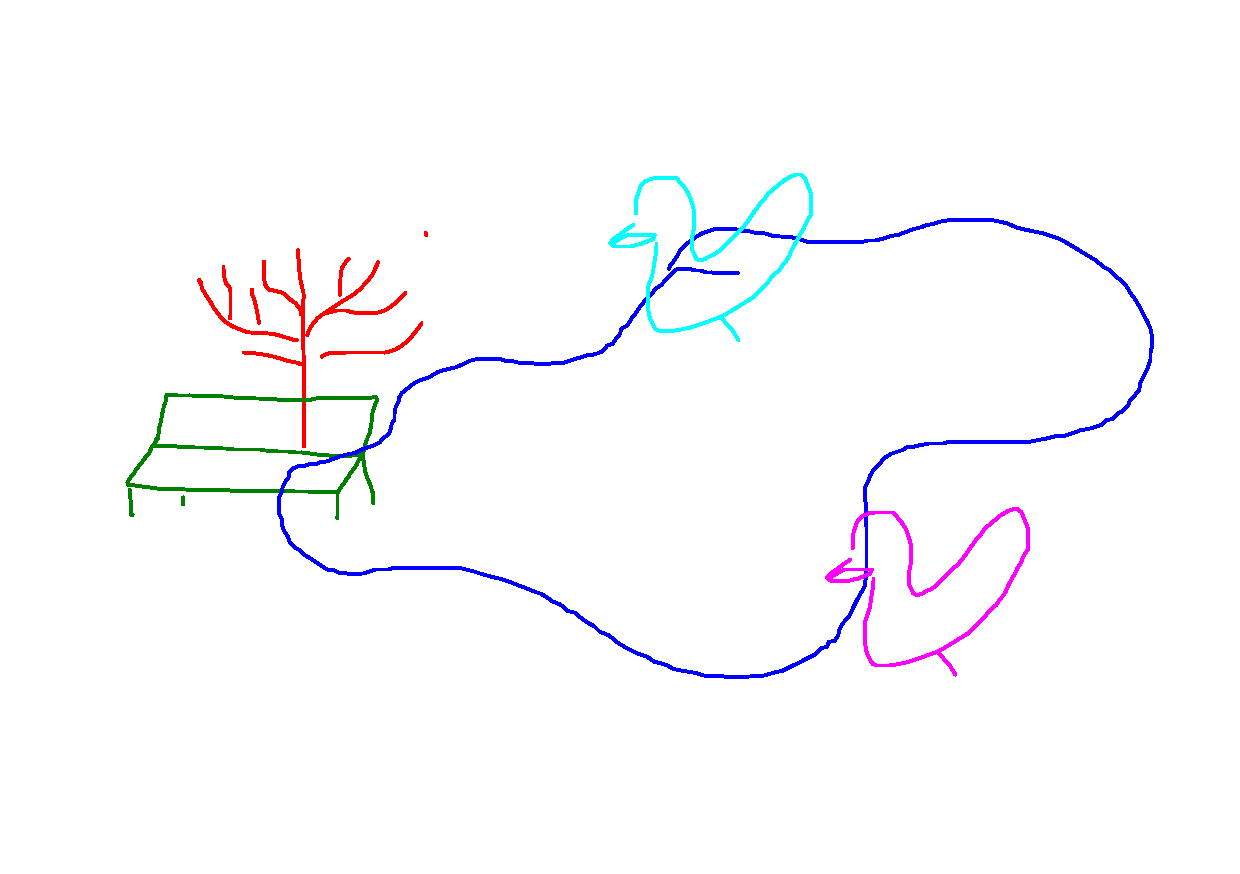
\includegraphics[width=\textwidth]{figures/drawing_2_cr.pdf}
                \caption{classifier-based constraints, relative sizes}
            \end{subfigure}
        \end{subfigure}
        \begin{subfigure}{\textwidth}
            \centering
            \caption{(3) \say{There is a house, and mountains behind it. The sun is rising above the mountains.}}
            \begin{subfigure}[t]{0.45\textwidth}
                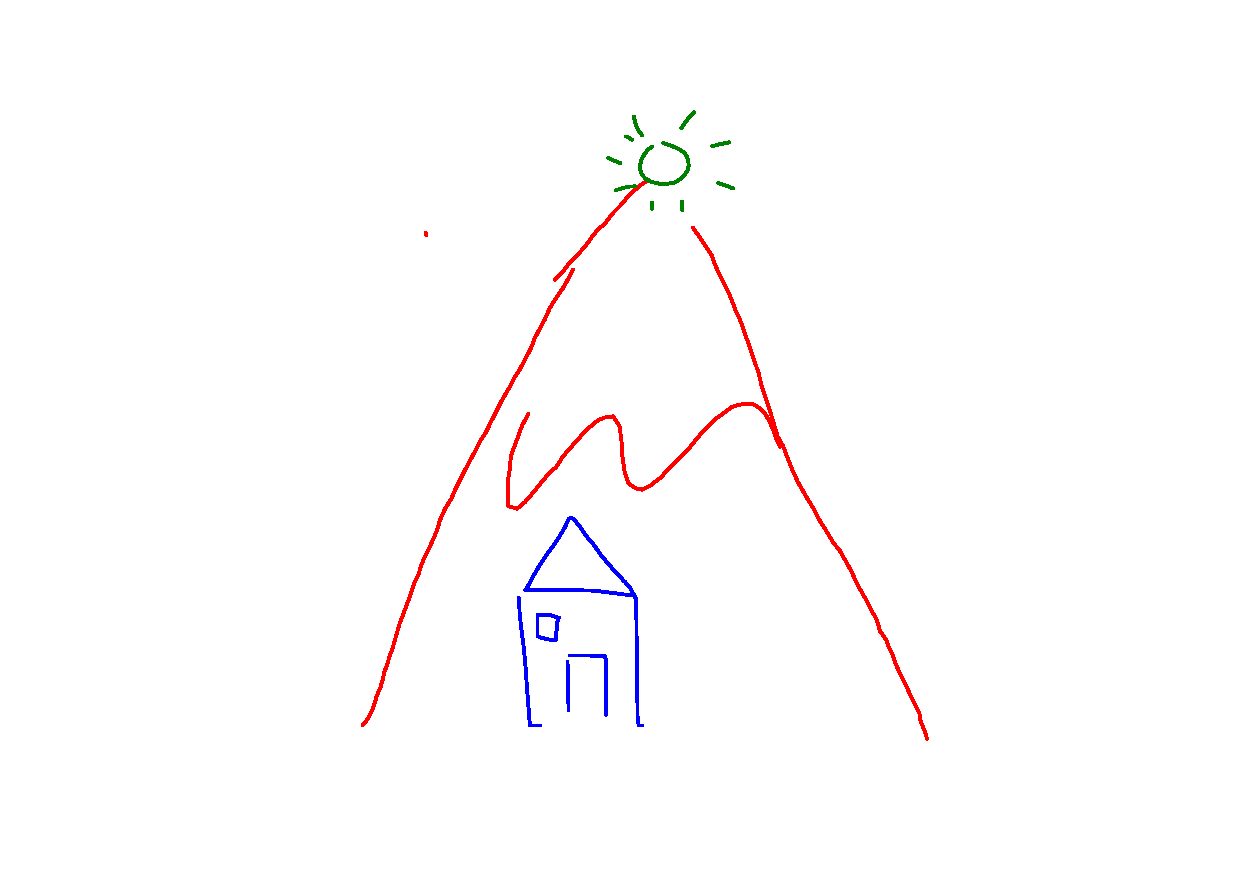
\includegraphics[width=\textwidth]{figures/drawing_3_rr.pdf} 
                \caption{rule-based constraints, relative sizes}
            \end{subfigure}
            \hfill
            \begin{subfigure}[t]{0.45\textwidth}
                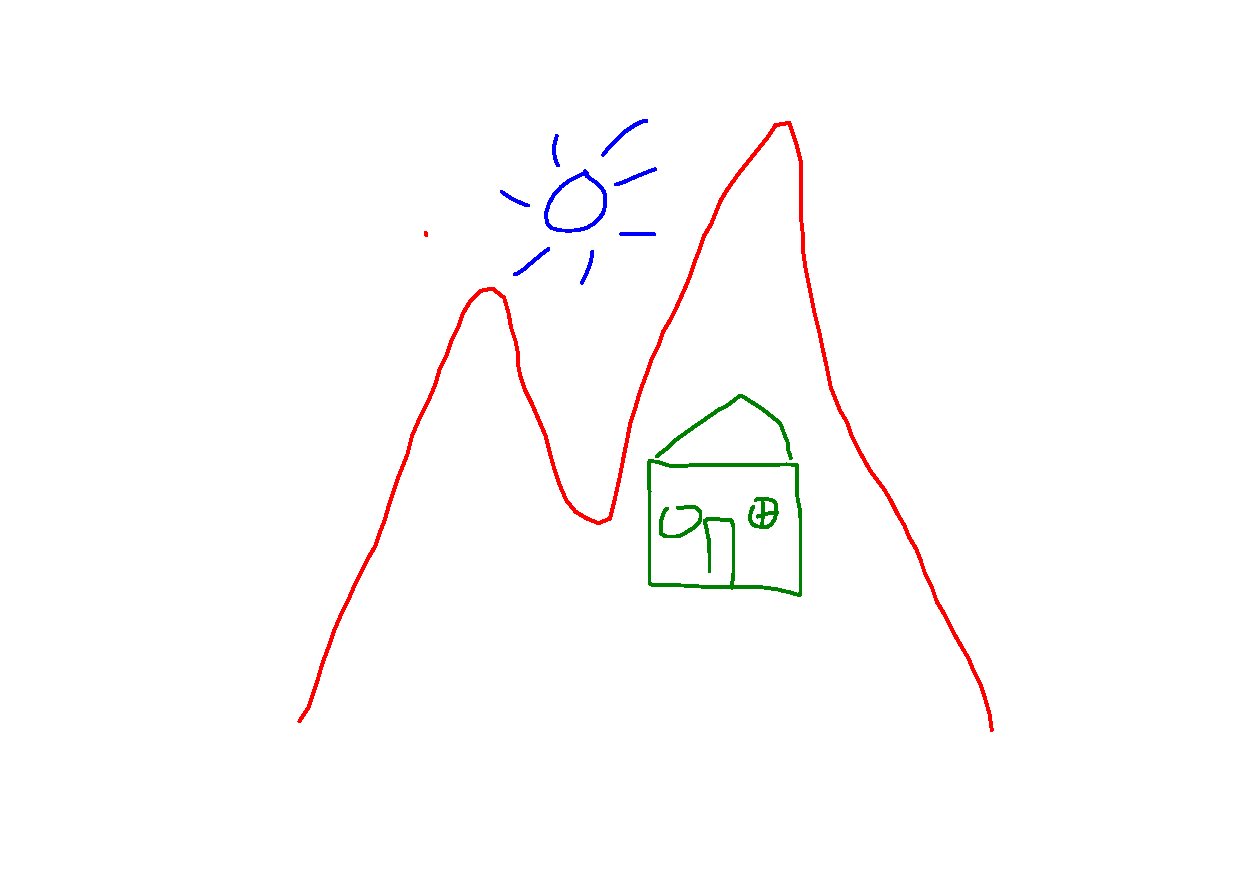
\includegraphics[width=\textwidth]{figures/drawing_3_cr.pdf}
                \caption{classifier-based constraints, relative sizes}
            \end{subfigure}
        \end{subfigure}
    \caption[Examples of generated drawings]{Examples of generated drawings. Each example is labelled with the used approach for determining the position and size. The absolute sizes refer to the hand crafted absolute size table.}
    \label{fig:composed_drawings}
\end{figure}

\chapter*{Conclusion}
\addcontentsline{toc}{chapter}{Conclusion}

In this thesis, we have developed a command-line and a web-based application that generates drawings from a textual description using scene graphs as an intermediate structure. We have proposed various approaches for determining the sizes and positions of objects in a scene based on their relations in the scene graph. We have shown that our proposed approach, in many cases, can generate drawings that correspond to the description. 

\medskip

Our approach may find their use in layout generation, used by some photorealistic image generators  \citep{zhao2019image}.  Photorealistic image generators that generate images using the scene graphs currently use box regression networks for this task \citep{johnson2018image,tripathi2019using}. Our approach could be an alternative to the box regression method. However, comparison with the box regression networks is beyond the scope of this thesis, and it may be a subject of future work.



%%% Bibliography
%%% Bibliography (literature used as a source)
%%%
%%% We employ bibTeX to construct the bibliography. It processes
%%% citations in the text (e.g., the \cite{...} macro) and looks up
%%% relevant entries in the bibliography.bib file.
%%%
%%% The \bibliographystyle command selects, which style will be used
%%% for references from the text. The argument in curly brackets is
%%% the name of the corresponding style file (*.bst). Both styles
%%% mentioned in this template are included in LaTeX distributions.

% \bibliographystyle{plainnat}    %% Author (year)
\bibliographystyle{unsrt}     %% [number]

\renewcommand{\bibname}{Bibliography}

%%% Generate the bibliography. Beware that if you cited no works,
%%% the empty list will be omitted completely.

\bibliography{bibliography}

%%% If case you prefer to write the bibliography manually (without bibTeX),
%%% you can use the following. Please follow the ISO 690 standard and
%%% citation conventions of your field of research.

% \begin{thebibliography}{99}
%
% \bibitem{lamport94}
%   {\sc Lamport,} Leslie.
%   \emph{\LaTeX: A Document Preparation System}.
%   2nd edition.
%   Massachusetts: Addison Wesley, 1994.
%   ISBN 0-201-52983-1.
%
% \end{thebibliography}


%%% Figures used in the thesis (consider if this is needed)
\listoffigures

%%% Tables used in the thesis (consider if this is needed)
%%% In mathematical theses, it could be better to move the list of tables to the beginning of the thesis.
\listoftables

%%% Abbreviations used in the thesis, if any, including their explanation
%%% In mathematical theses, it could be better to move the list of abbreviations to the beginning of the thesis.
%\chapwithtoc{List of Abbreviations}

%%% Attachments to the bachelor thesis, if any. Each attachment must be
%%% referred to at least once from the text of the thesis. Attachments
%%% are numbered.
%%%
%%% The printed version should preferably contain attachments, which can be
%%% read (additional tables and charts, supplementary text, examples of
%%% program output, etc.). The electronic version is more suited for attachments
%%% which will likely be used in an electronic form rather than read (program
%%% source code, data files, interactive charts, etc.). Electronic attachments
%%% should be uploaded to SIS and optionally also included in the thesis on a~CD/DVD.
%%% Allowed file formats are specified in provision of the rector no. 72/2017.
\appendix
\chapter{Attachments}

\section{Source Code}
\label{attachment:sources}

Zipped source code that contains:
\begin{itemize}
\item implementation of the command-line interface, web server in the \verb|drawtomat| directory; 
\item implementation of the web client in the \verb|web| directory;
\item various experiments and scripts used for training the used models in the \verb|experiments| directory. 
\end{itemize}
The source code is also available as a GitHub repository \url{https://github.com/peter-grajcar/ drawtomat}.

\openright
\end{document}